% !TeX spellcheck = en_GB

\section{Algorithms}\label{algorithms}
\subsection{Sub modules} \label{subModules}
Sub modules are parts of the algorithms that are denoted circled with \circled{A}, \circled{B}, \circled{C}, \circled{D} and \circled{E}. They are procedures that will be explained in more detail for a better understanding of the way of working of algorithms in the following chapters. \circled{E} is explained not until Chapter \ref{var2} because it is needed only there.\\

\noindent \textbf{Distribute$(\Sigma,\ V) $ \circled{A} and Distribute$(V^2,\ V)$ \circled{B}:}\\
The difference between \circled{A} and \circled{B} is that one time $\Sigma$ and the other time $V^2$ are distributed. But in both cases a uniform random subset of the $Rhse$ is taken and again uniform randomly distributed over the set of available variables $V$. While distributing the terminals there exists at least one rule for every terminal used in the word $w$. The specifics of how they are distributed are described in the following algorithm: \\

\noindent
\frame{
	\begin{algorithm}[H] %or another one check
		\caption{Distribute}
		\label{Distribute}
		\SetAlgoLined
		\KwIn{$V,~Rhse \subseteq\ V^{2}~or~Rhse \subseteq \Sigma$}
		\KwOut{Set of productions $P \subseteq V \times V^{2}$ or $P \subseteq V \times \Sigma$}
		\ForEach{$rhse \in Rhse$}{
			$choose\ n\ uniformly\ randomly\ in\ [i, j]$;~~\tcp{$i \in  \mathbb{N},\ j \in  \mathbb{N}$}
			$V_{add} := uniform\ random\ subset\ of\ size\ n\ from\ V$\; \label{sizeN}
			$P \cup \{ (v, rhse)\ |\ v \in V_{add},\ rhse \in Rhse \} $\;	
		}
		\Return $P$;
	\end{algorithm}
} \\

\noindent \textbf{Stopping Criteria \circled{C}:}\\
Two kinds of stopping criteria are used to determine whether an algorithm should terminate early on because an already suitable exercise has been found:
\begin{itemize}[noitemsep,nolistsep]
	\item stop if more than half of the pyramid cells are not empty any more
	\item stop if the root of the pyramid is not empty any more
\end{itemize}
Both stopping criteria are compared in Chapter \ref{AnalysisOfAlgorithms} to see which one leads to more suitable exam $exercises$. \\
\pagebreak

\noindent \textbf{CalculateSubsetForCell(Pyramid, i, j) \circled{D}:}\\
This procedure is needed to determine all possible compound variables out of all possible cell combinations for one specific cell. It works kind of analogous from Line 7 to Line 9 of the CYK algorithm (Algorithm \ref{CYK}).\\

\noindent \frame{
	\begin{algorithm}[H] %or another one check
		\caption{CalculateSubsetForCell}
		\label{CalculateSubsetForCell}
		\SetAlgoLined
		\KwIn{$Pyramid,~i \in  \mathbb{N},\ j \in  \mathbb{N}$ }
		\KwOut{$CellSet \subseteq V^2$}
		$CellSet=\emptyset$\;
		\For{$k:=i-1 \to 0$}{ \label{cellCombs}
			$CellSet \cup \{YZ\ |\ X\longrightarrow YZ,\ Y \in Cell_{k,j},\ Z \in Cell_{i-k-1,k+j+1} \}$\; \label{cellSet}
		}
		\Return $CellSet$;
		
	\end{algorithm}
}
In the following situation a rule is added to $Cell_{3,0}$ while using Algorithm \ref{CalculateSubsetForCell}.
\noindent
\begin{figure}[h]
	\begin{minipage}{6in}
		\centering
		\raisebox{-0.5\height}{
			\begin{tabular}{l}
				Grammar:\\
				$A \rightarrow AB~|~a$\\
				$\mathbf{B \rightarrow \textbf{SC}}~|~b$\\ 
				$C \rightarrow AB$ \\
				$S \rightarrow BA~|~AA$
			\end{tabular} 
		}
		\hspace*{.2in}
		\raisebox{-0.5\height}{
			\resizebox{0.5\linewidth}{!}{
				\resizebox{\linewidth}{!}{
					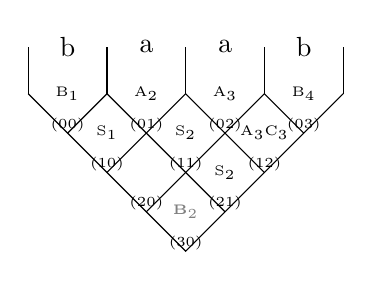
\begin{tikzpicture}[baseline]
					\newcommand{\myfontvars}[1]{
						\fontsize{4.9}{12}\selectfont{#1}
					}\newcommand{\myfontnumbering}[1]{
						\fontsize{2.5}{12}\selectfont{#1}
					}%Outer hull
					%Tip of the pyramid
					\coordinate (tip) at (2.0,-2.0);
					\foreach \i in {0,...,4} {
						\coordinate (\i) at (\i,0);
					}
					%Draw the left and right line of the pyramid pointing downwards
					\draw (0) -- (tip) -- (4);
					%Grid lines direction down-left to top-right
					\coordinate (dl1) at (0.5,-0.5);
					\coordinate (dl2) at (1.0,-1.0);
					\coordinate (dl3) at (1.5,-1.5);
					\draw (dl1) -- (1,0);
					\draw (dl2) -- (2,0);
					\draw (dl3) -- (3,0);
					%Grid lines direction down-right to top-left
					\coordinate (dr1) at (2.5,-1.5);
					\coordinate (dr2) at (3.0,-1.0);
					\coordinate (dr3) at (3.5,-0.5);
					\draw (dr1) -- (1,0);
					\draw (dr2) -- (2,0);
					\draw (dr3) -- (3,0);
					%Small lines at the top
					\coordinate (top0) at (0.0,0.0);
					\coordinate (top1) at (1.0,0.0);
					\coordinate (top2) at (2.0,0.0);
					\coordinate (top3) at (3.0,0.0);
					\coordinate (top4) at (4.0,0.0);
					\coordinate (topUpper0) at (0.0,0.6);
					\coordinate (topUpper1) at (1.0,0.6);
					\coordinate (topUpper2) at (2.0,0.6);
					\coordinate (topUpper3) at (3.0,0.6);
					\coordinate (topUpper4) at (4.0,0.6);
					\draw (top0) -- (topUpper0);
					\draw (top1) -- (topUpper1);
					\draw (top2) -- (topUpper2);
					\draw (top3) -- (topUpper3);
					\draw (top4) -- (topUpper4);
					%The string
					\coordinate (w0) at (0.5,0.6);
					\coordinate (w1) at (1.5,0.6);
					\coordinate (w2) at (2.5,0.6);
					\coordinate (w3) at (3.5,0.6);
					\node [] at (w0) {b};
					\node [] at (w1) {a};
					\node [] at (w2) {a};
					\node [] at (w3) {b};
					% Variables in the cells
					%cells00
					\coordinate (center00) at (0.5,0.0);
					\node [below=0.18cm] at (center00) {\myfontnumbering{$(00)$}};
					\node [] at (center00) {\myfontvars{B$_{1}$}};
					%cells01
					\coordinate (center01) at (1.5,0.0);
					\node [below=0.18cm] at (center01) {\myfontnumbering{$(01)$}};
					\node [] at (center01) {\myfontvars{A$_{2}$}};
					%cells02
					\coordinate (center02) at (2.5,0.0);
					\node [below=0.18cm] at (center02) {\myfontnumbering{$(02)$}};
					\node [] at (center02) {\myfontvars{A$_{3}$}};
					%cells03
					\coordinate (center03) at (3.5,0.0);
					\node [below=0.18cm] at (center03) {\myfontnumbering{$(03)$}};
					\node [] at (center03) {\myfontvars{B$_{4}$}};
					%cells10
					\coordinate (center10) at (1.0,-0.5);
					\node [below=0.18cm] at (center10) {\myfontnumbering{$(10)$}};
					\node [] at (center10) {\myfontvars{S$_{1}$}};
					%cells11
					\coordinate (center11) at (2.0,-0.5);
					\node [below=0.18cm] at (center11) {\myfontnumbering{$(11)$}};
					\node [] at (center11) {\myfontvars{S$_{2}$}};
					%cells12
					\coordinate (center12) at (3.0,-0.5);
					\node [below=0.18cm] at (center12) {\myfontnumbering{$(12)$}};
					\node [] at (center12) {\myfontvars{A$_{3}$C$_{3}$}};
					%cells20
					\coordinate (center20) at (1.5,-1.0);
					\node [below=0.18cm] at (center20) {\myfontnumbering{$(20)$}};
					%cells21
					\coordinate (center21) at (2.5,-1.0);
					\node [below=0.18cm] at (center21) {\myfontnumbering{$(21)$}};
					\node [] at (center21) {\myfontvars{S$_{2}$}};
					%cells30
					\coordinate (center30) at (2.0,-1.5);
					\node [below=0.18cm] at (center30) {\myfontnumbering{$(30)$}};
					\node [] at (center30) {\myfontvars{\textcolor{gray}{\textbf{B$_{2}$}}}};
					\end{tikzpicture}
				}	
			}
		}
	\end{minipage}
	\caption{Example of Algorithm \ref{CalculateSubsetForCell} while applying it on $Cell_{3,0}$ via adding the rule $B \rightarrow SC$.}
\end{figure}\\
The calculation of CellSet for $Cell_{3,0}$ results in $\{SA,~SC,~BS\}$, whereas $SA$ and $SC$ stem from $Cell_{1,0}$ together with $Cell_{1,2}$ and $BA$ comes from $Cell_{0,0}$ together with $Cell_{2,1}$. Now if either one of the rules $lhse \rightarrow SA$, $lhse \rightarrow SC$ or  $lhse \rightarrow BS$ is added to the grammar, then $lhse\in Cell_{3,0}$. Here the rule  \textbf{B $\rightarrow$ SC} has been added and finally $(B,2)$ is element of $Cell_{3,0}$.\\
In general if for one $Cell_{i,j}$ a rule like $lhse \rightarrow cs$ with $cs \in CellSet~(Line~\ref{cellSet})$ is added then automatically $Cell_{i,j}$ won't be empty any more. 
\pagebreak

\subsection{Dice rolling the distributions only} \label{diceRollOnlyCYK}
\noindent We start off by a primitive way of generating grammars, which will be the lower boundary while comparing the algorithms. Note that later on in Chapter \ref{successRates} it is described what "performing better" means in the context of this thesis. \\

\noindent
\frame{
	\begin{algorithm}[H] %or another one check
		\caption{DiceRollOnlyCYK}
		\label{DiceRollOnlyCYK}
		\SetAlgoLined
		\KwIn{Word $w \in \Sigma^{*}$ }
		\KwOut{Set of productions $P$}
		$P = \emptyset$;~~\tcp{$P \subseteq V \times (V^{2} \cup \Sigma)$}
		$P = Distribute(\Sigma,\ V)$;  \circled{A}\\ \label{diceRollOnlyA}
		$P \cup Distribute(V^2,\ V)$;  \circled{B}\\ \label{diceRollOnlyB}
		\Return $P$;
	\end{algorithm}
}
The algoritm DiceRollOnly (Algorithm \ref{DiceRollOnlyCYK}) distributes terminals $\Sigma$ to at least one $lhse$, but a compound variable $V^2$ does not has to be distributed at all. Note that for each terminal of $\Sigma=\{a,b\}$ at least one rule like $lhse\rightarrow a$ and $lhse\rightarrow b$ is generated. But for each possible compound variable $V^2=\{AA,~AB,~AC,~AS,~BB,~BC,~BS,~CC,$ $~CS,SS\}$ it is possible that only a smaller subset like $\{AA,~BA,~CC,~SC\}$ is distributed so that only rules like $lhse\rightarrow AA$, $lhse\rightarrow BA$, $lhse\rightarrow CC$ and $lhse\rightarrow SC$ exist.
\noindent
\begin{figure} [h]
	\begin{minipage}{6in}
		\centering
		\raisebox{-0.5\height}{
		\begin{tabular}{l}
				Grammar after Line 2:\\
				$C\rightarrow a$\\ 
				$B\rightarrow b$\\
				\\
			\end{tabular} 
		\begin{tabular}{l}
			Grammar after Line 3:\\
			$C\rightarrow BA~|~AA~|~a$\\ 
			$B\rightarrow b$ \\
			$S\rightarrow CC~|~SC$ 
		\end{tabular}
	} 		
	\end{minipage}
	\caption{Shortend overview of an example of Algorithm \ref{DiceRollOnlyCYK} as described before.}
	\label{DiceRollONlyCYKExample}
\end{figure}
\pagebreak
\clearpage
\subsection{Dice rolling and Bottom-Up variant one}
Another approach to design an algorithm is after the Bottom-Up approach (Chapter \ref{approaches}) in which the parsing table is filled starting from the leaves in direction of the root node.\\
The basic idea is to guide the choice of rules while distributing the compound variables $V^2$. In Algorithm \ref{DiceRollOnlyCYK}, the naive approach, it is possible that the terminals are distributed to the variables $A$ and $B$ and Algorithm \ref{DiceRollOnlyCYK} completely discards this fact during the distribution of the compound variables (see Figure \ref{var1Example}, the middle part of the example). \\
\noindent
\begin{figure}[h]
	\begin{minipage}{6in}
		\centering
		\raisebox{-0.5\height}{
			\begin{tabular}{l}
				Grammar:\\
				$A\rightarrow a$\\
				$B \rightarrow b$\\ 
			\end{tabular} 
		}
		\hspace*{.2in}
			\resizebox{0.5\linewidth}{!}{
				\resizebox{\linewidth}{!}{
					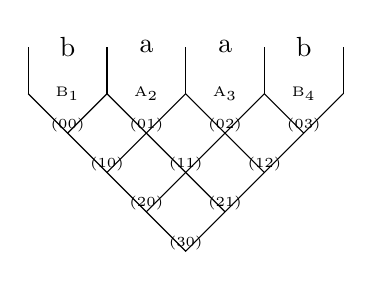
\begin{tikzpicture}[baseline]
					\newcommand{\myfontvars}[1]{
						\fontsize{4.9}{12}\selectfont{#1}
					}\newcommand{\myfontnumbering}[1]{
						\fontsize{2.5}{12}\selectfont{#1}
					}%Outer hull
					%Tip of the pyramid
					\coordinate (tip) at (2.0,-2.0);
					\foreach \i in {0,...,4} {
						\coordinate (\i) at (\i,0);
					}
					%Draw the left and right line of the pyramid pointing downwards
					\draw (0) -- (tip) -- (4);
					%Grid lines direction down-left to top-right
					\coordinate (dl1) at (0.5,-0.5);
					\coordinate (dl2) at (1.0,-1.0);
					\coordinate (dl3) at (1.5,-1.5);
					\draw (dl1) -- (1,0);
					\draw (dl2) -- (2,0);
					\draw (dl3) -- (3,0);
					%Grid lines direction down-right to top-left
					\coordinate (dr1) at (2.5,-1.5);
					\coordinate (dr2) at (3.0,-1.0);
					\coordinate (dr3) at (3.5,-0.5);
					\draw (dr1) -- (1,0);
					\draw (dr2) -- (2,0);
					\draw (dr3) -- (3,0);
					%Small lines at the top
					\coordinate (top0) at (0.0,0.0);
					\coordinate (top1) at (1.0,0.0);
					\coordinate (top2) at (2.0,0.0);
					\coordinate (top3) at (3.0,0.0);
					\coordinate (top4) at (4.0,0.0);
					\coordinate (topUpper0) at (0.0,0.6);
					\coordinate (topUpper1) at (1.0,0.6);
					\coordinate (topUpper2) at (2.0,0.6);
					\coordinate (topUpper3) at (3.0,0.6);
					\coordinate (topUpper4) at (4.0,0.6);
					\draw (top0) -- (topUpper0);
					\draw (top1) -- (topUpper1);
					\draw (top2) -- (topUpper2);
					\draw (top3) -- (topUpper3);
					\draw (top4) -- (topUpper4);
					%The string
					\coordinate (w0) at (0.5,0.6);
					\coordinate (w1) at (1.5,0.6);
					\coordinate (w2) at (2.5,0.6);
					\coordinate (w3) at (3.5,0.6);
					\node [] at (w0) {b};
					\node [] at (w1) {a};
					\node [] at (w2) {a};
					\node [] at (w3) {b};
					% Variables in the cells
					%cells00
					\coordinate (center00) at (0.5,0.0);
					\node [below=0.18cm] at (center00) {\myfontnumbering{$(00)$}};
					\node [] at (center00) {\myfontvars{B$_{1}$}};
					%cells01
					\coordinate (center01) at (1.5,0.0);
					\node [below=0.18cm] at (center01) {\myfontnumbering{$(01)$}};
					\node [] at (center01) {\myfontvars{A$_{2}$}};
					%cells02
					\coordinate (center02) at (2.5,0.0);
					\node [below=0.18cm] at (center02) {\myfontnumbering{$(02)$}};
					\node [] at (center02) {\myfontvars{A$_{3}$}};
					%cells03
					\coordinate (center03) at (3.5,0.0);
					\node [below=0.18cm] at (center03) {\myfontnumbering{$(03)$}};
					\node [] at (center03) {\myfontvars{B$_{4}$}};
					%cells10
					\coordinate (center10) at (1.0,-0.5);
					\node [below=0.18cm] at (center10) {\myfontnumbering{$(10)$}};
					%cells11
					\coordinate (center11) at (2.0,-0.5);
					\node [below=0.18cm] at (center11) {\myfontnumbering{$(11)$}};
					%cells12
					\coordinate (center12) at (3.0,-0.5);
					\node [below=0.18cm] at (center12) {\myfontnumbering{$(12)$}};
					%cells20
					\coordinate (center20) at (1.5,-1.0);
					\node [below=0.18cm] at (center20) {\myfontnumbering{$(20)$}};
					%cells21
					\coordinate (center21) at (2.5,-1.0);
					\node [below=0.18cm] at (center21) {\myfontnumbering{$(21)$}};
					%cells30
					\coordinate (center30) at (2.0,-1.5);
					\node [below=0.18cm] at (center30) {\myfontnumbering{$(30)$}};
					\end{tikzpicture}
				}	
			}
\begin{minipage}{6in}
		\centering
		\raisebox{-0.5\height}{
		\begin{tabular}{l}
			Grammar:\\
			$A\rightarrow \mathbf{CC}~|~a$\\
			$B \rightarrow b$\\ 
		\end{tabular} 
	}
\hspace*{.2in}
\resizebox{0.5\linewidth}{!}{
\resizebox{\linewidth}{!}{
	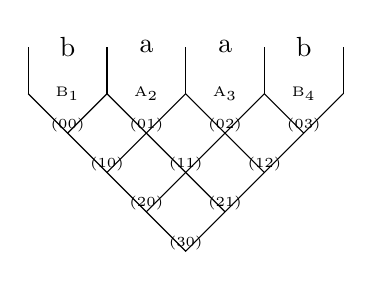
\begin{tikzpicture}[baseline]
	\newcommand{\myfontvars}[1]{
		\fontsize{4.9}{12}\selectfont{#1}
	}\newcommand{\myfontnumbering}[1]{
		\fontsize{2.5}{12}\selectfont{#1}
	}%Outer hull
	%Tip of the pyramid
	\coordinate (tip) at (2.0,-2.0);
	\foreach \i in {0,...,4} {
		\coordinate (\i) at (\i,0);
	}
	%Draw the left and right line of the pyramid pointing downwards
	\draw (0) -- (tip) -- (4);
	%Grid lines direction down-left to top-right
	\coordinate (dl1) at (0.5,-0.5);
	\coordinate (dl2) at (1.0,-1.0);
	\coordinate (dl3) at (1.5,-1.5);
	\draw (dl1) -- (1,0);
	\draw (dl2) -- (2,0);
	\draw (dl3) -- (3,0);
	%Grid lines direction down-right to top-left
	\coordinate (dr1) at (2.5,-1.5);
	\coordinate (dr2) at (3.0,-1.0);
	\coordinate (dr3) at (3.5,-0.5);
	\draw (dr1) -- (1,0);
	\draw (dr2) -- (2,0);
	\draw (dr3) -- (3,0);
	%Small lines at the top
	\coordinate (top0) at (0.0,0.0);
	\coordinate (top1) at (1.0,0.0);
	\coordinate (top2) at (2.0,0.0);
	\coordinate (top3) at (3.0,0.0);
	\coordinate (top4) at (4.0,0.0);
	\coordinate (topUpper0) at (0.0,0.6);
	\coordinate (topUpper1) at (1.0,0.6);
	\coordinate (topUpper2) at (2.0,0.6);
	\coordinate (topUpper3) at (3.0,0.6);
	\coordinate (topUpper4) at (4.0,0.6);
	\draw (top0) -- (topUpper0);
	\draw (top1) -- (topUpper1);
	\draw (top2) -- (topUpper2);
	\draw (top3) -- (topUpper3);
	\draw (top4) -- (topUpper4);
	%The string
	\coordinate (w0) at (0.5,0.6);
	\coordinate (w1) at (1.5,0.6);
	\coordinate (w2) at (2.5,0.6);
	\coordinate (w3) at (3.5,0.6);
	\node [] at (w0) {b};
	\node [] at (w1) {a};
	\node [] at (w2) {a};
	\node [] at (w3) {b};
	% Variables in the cells
	%cells00
	\coordinate (center00) at (0.5,0.0);
	\node [below=0.18cm] at (center00) {\myfontnumbering{$(00)$}};
	\node [] at (center00) {\myfontvars{B$_{1}$}};
	%cells01
	\coordinate (center01) at (1.5,0.0);
	\node [below=0.18cm] at (center01) {\myfontnumbering{$(01)$}};
	\node [] at (center01) {\myfontvars{A$_{2}$}};
	%cells02
	\coordinate (center02) at (2.5,0.0);
	\node [below=0.18cm] at (center02) {\myfontnumbering{$(02)$}};
	\node [] at (center02) {\myfontvars{A$_{3}$}};
	%cells03
	\coordinate (center03) at (3.5,0.0);
	\node [below=0.18cm] at (center03) {\myfontnumbering{$(03)$}};
	\node [] at (center03) {\myfontvars{B$_{4}$}};
	%cells10
	\coordinate (center10) at (1.0,-0.5);
	\node [below=0.18cm] at (center10) {\myfontnumbering{$(10)$}};
	%cells11
	\coordinate (center11) at (2.0,-0.5);
	\node [below=0.18cm] at (center11) {\myfontnumbering{$(11)$}};
	%cells12
	\coordinate (center12) at (3.0,-0.5);
	\node [below=0.18cm] at (center12) {\myfontnumbering{$(12)$}};
	%cells20
	\coordinate (center20) at (1.5,-1.0);
	\node [below=0.18cm] at (center20) {\myfontnumbering{$(20)$}};
	%cells21
	\coordinate (center21) at (2.5,-1.0);
	\node [below=0.18cm] at (center21) {\myfontnumbering{$(21)$}};
	%cells30
	\coordinate (center30) at (2.0,-1.5);
	\node [below=0.18cm] at (center30) {\myfontnumbering{$(30)$}};
	\end{tikzpicture}
}	
}
\end{minipage}
\begin{minipage}{6in}
\centering
\raisebox{-0.5\height}{
	\begin{tabular}{l}
		Grammar:\\
		$A\rightarrow a$\\
		$B \rightarrow \mathbf{AB}~|~b$\\ 
	\end{tabular} 
}
\hspace*{.2in}
\resizebox{0.5\linewidth}{!}{
	\resizebox{\linewidth}{!}{
		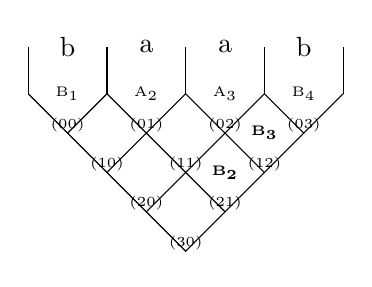
\begin{tikzpicture}[baseline]
		\newcommand{\myfontvars}[1]{
			\fontsize{4.9}{12}\selectfont{#1}
		}\newcommand{\myfontnumbering}[1]{
			\fontsize{2.5}{12}\selectfont{#1}
		}%Outer hull
		%Tip of the pyramid
		\coordinate (tip) at (2.0,-2.0);
		\foreach \i in {0,...,4} {
			\coordinate (\i) at (\i,0);
		}
		%Draw the left and right line of the pyramid pointing downwards
		\draw (0) -- (tip) -- (4);
		%Grid lines direction down-left to top-right
		\coordinate (dl1) at (0.5,-0.5);
		\coordinate (dl2) at (1.0,-1.0);
		\coordinate (dl3) at (1.5,-1.5);
		\draw (dl1) -- (1,0);
		\draw (dl2) -- (2,0);
		\draw (dl3) -- (3,0);
		%Grid lines direction down-right to top-left
		\coordinate (dr1) at (2.5,-1.5);
		\coordinate (dr2) at (3.0,-1.0);
		\coordinate (dr3) at (3.5,-0.5);
		\draw (dr1) -- (1,0);
		\draw (dr2) -- (2,0);
		\draw (dr3) -- (3,0);
		%Small lines at the top
		\coordinate (top0) at (0.0,0.0);
		\coordinate (top1) at (1.0,0.0);
		\coordinate (top2) at (2.0,0.0);
		\coordinate (top3) at (3.0,0.0);
		\coordinate (top4) at (4.0,0.0);
		\coordinate (topUpper0) at (0.0,0.6);
		\coordinate (topUpper1) at (1.0,0.6);
		\coordinate (topUpper2) at (2.0,0.6);
		\coordinate (topUpper3) at (3.0,0.6);
		\coordinate (topUpper4) at (4.0,0.6);
		\draw (top0) -- (topUpper0);
		\draw (top1) -- (topUpper1);
		\draw (top2) -- (topUpper2);
		\draw (top3) -- (topUpper3);
		\draw (top4) -- (topUpper4);
		%The string
		\coordinate (w0) at (0.5,0.6);
		\coordinate (w1) at (1.5,0.6);
		\coordinate (w2) at (2.5,0.6);
		\coordinate (w3) at (3.5,0.6);
		\node [] at (w0) {b};
		\node [] at (w1) {a};
		\node [] at (w2) {a};
		\node [] at (w3) {b};
		% Variables in the cells
		%cells00
		\coordinate (center00) at (0.5,0.0);
		\node [below=0.18cm] at (center00) {\myfontnumbering{$(00)$}};
		\node [] at (center00) {\myfontvars{B$_{1}$}};
		%cells01
		\coordinate (center01) at (1.5,0.0);
		\node [below=0.18cm] at (center01) {\myfontnumbering{$(01)$}};
		\node [] at (center01) {\myfontvars{A$_{2}$}};
		%cells02
		\coordinate (center02) at (2.5,0.0);
		\node [below=0.18cm] at (center02) {\myfontnumbering{$(02)$}};
		\node [] at (center02) {\myfontvars{A$_{3}$}};
		%cells03
		\coordinate (center03) at (3.5,0.0);
		\node [below=0.18cm] at (center03) {\myfontnumbering{$(03)$}};
		\node [] at (center03) {\myfontvars{B$_{4}$}};
		%cells10
		\coordinate (center10) at (1.0,-0.5);
		\node [below=0.18cm] at (center10) {\myfontnumbering{$(10)$}};
		%cells11
		\coordinate (center11) at (2.0,-0.5);
		\node [below=0.18cm] at (center11) {\myfontnumbering{$(11)$}};
		%cells12
		\coordinate (center12) at (3.0,-0.5);
		\node [below=0.18cm] at (center12) {\myfontnumbering{$(12)$}};
		\node [] at (center12) {\myfontvars{\textbf{B}$\mathbf{_{3}}$}};
		%cells20
		\coordinate (center20) at (1.5,-1.0);
		\node [below=0.18cm] at (center20) {\myfontnumbering{$(20)$}};
		%cells21
		\coordinate (center21) at (2.5,-1.0);
		\node [below=0.18cm] at (center21) {\myfontnumbering{$(21)$}};
		\node [] at (center21) {\myfontvars{\textbf{B}$\mathbf{_{2}}$}};
		%cells30
		\coordinate (center30) at (2.0,-1.5);
		\node [below=0.18cm] at (center30) {\myfontnumbering{$(30)$}};
		\end{tikzpicture}
	}	
}
\end{minipage}	
\end{minipage}
	\caption{Example of disregarding the already added rules. Top: starting situation. Middle: Unfortunate adding of rules that doesn't help to fill the parsing table and can happen in Algorithm \ref{DiceRollOnlyCYK}. Bottom: Good adding of rules as intended in Algorithm \ref{BottomUpDiceRollVar1} that helps filling.}
	\label{var1Example}
\end{figure}\\
If rules like $lhse \rightarrow CC$ or $lhse \rightarrow SC$ are added they don't directly help to fill the parsing table and bloat the grammar with useless rules (see Figure \ref{var1Example}, the middle part of the example). More reasonable rules to add would be $lhse \rightarrow BA$, $lhse \rightarrow AA$ or $lhse \rightarrow AB$ (see Figure \ref{var1Example}, the bottom part of the example).\\
\noindent Algorithm \ref{BottomUpDiceRollVar1} continues on this idea: After distributing the terminals (Line \ref{distrTerm}) the updated parsing table (Line \ref{var1Update}) is always taken into consideration while calculating (Line \ref{var1D}) variable compounds and to finally add a part of them (Line \ref{var1Add}) in form of rules to the grammar. In explanation  for each chosen cell a $CellSet$ (Line \ref{var1D}) is calculated, that only contains reasonable variable compounds. This way only variable compounds are added that directly help to fill the parsing table.\\

\noindent
\frame{
	\begin{algorithm}[H] %or another one check
		\caption{BottomUpDiceRollVar1}
		\label{BottomUpDiceRollVar1}
		\SetAlgoLined
		\KwIn{Word $w \in \Sigma^{*}$ }
		\KwOut{Set of productions $P$}
		$P = \emptyset$;~~\tcp{$P \subseteq V \times (V^{2} \cup \Sigma)$}
		$P = Distribute(\Sigma,\ V)$;  \circled{A} \label{distrTerm}\\
		$Pyramid = CYK(G,\ w)$\label{var1Stepii}\;
		\For{$i:=1\ \textbf{to}\ i_{max}$}{
			$J = \{0,~...~,~j_{max} -1\}$;~~\tcp{$J \subseteq \mathbb{N}$}
			$CellSet = \emptyset$;~~\tcp{$CellSet \subseteq V^2$} \label{var1A}
			\While{$|J|>0$}{
				$choose\ one\ j \in J\ uniform\ randomly$\;
				$J = J \setminus \{j\} $\label{chooseJ}\;
				$CellSet = CalculateSubsetForCell(Pyramid,\ i,\ j)$;  \circled{D} \label{var1D}\\
				$P \cup Distribute(CellSet,\ V)$;  \circled{B} \label{var1Add}\\
				$Pyramid = CYK(G,\ w)$\; \label{var1Update}
				\If{$stopping\ criteria~met$~\circled{C}}{
					\Return $P$\;
				}
			}
		}
		\Return $P$\;
		\footnotetext{
			\noindent Line \ref{var1Stepii}: Fills the i=0 row of the pyramid.
			
			\noindent Line \ref{chooseJ}: A cell is visited only once.
		}
	\end{algorithm}
}

\pagebreak
\subsection{Dice rolling and Bottom-Up variant two} \label{var2}
While examining Algorithm \ref{BottomUpDiceRollVar1} via its log file (Figure \ref{logsVar1}) it can be seen that already a very small number of rules in the grammar is sufficient so that the stopping criteria \circled{C} is met \textendash~the cells that indirectly decide what rules to add are mostly from row one ($i=1$) and sometimes if at all from row two ($i=2$).\\

\begin{figure}[h]
	\centering
		\begin{tabular}{l}
			Final cell worked with Index: 1,2\\
			Final cell worked with Index: 1,0\\
			Final cell worked with Index: 1,6 \\
			Final cell worked with Index: 1,0\\
			Final cell worked with Index: 1,2\\
			Final cell worked with Index: 1,3\\
			Final cell worked with Index: 2,4\\
	\end{tabular}
	\caption{Digest of log files of Algorithm \ref{BottomUpDiceRollVar1} with $|V|=4$ and $|\Sigma|=2$.}
	\label{logsVar1}
\end{figure}
\noindent This again leads to a further improvement idea to introduce a row dependent $threshold_i$ (Line \ref{var2threshold} of Algorithm \ref{BottomUpDiceRollVar2} BottomUpDiceRollVars) which helps that more cells with $i\geq2$ are chosen \textendash~what possibly leads to more diverse grammars being generated. The diversity, in context of the procedure BottomUpDiceRollVar1 (Algorithm \ref{BottomUpDiceRollVar1}), is somewhat too restricted to the $lhse$s that have one of the terminals as its $rhse$. Most of the rules that are part of the grammar will contain one of these $lhse$s as explained in Figure \ref{var1Example}. This is caused by the basic idea of Algorithm \ref{BottomUpDiceRollVar1} but also due to the relatively small number of rules that are added to the grammar altogether. \\
Further diversification is achieved through the usage of \circled{E} (Line \ref{chooseVc} of Algorithm \ref{BottomUpDiceRollVar2} BottomUpDiceRollVars), i.e. the variable compounds that already have been used in a row with low index $i$ are at a disadvantage to be picked again (A more detailed explanation is found at the and of this chapter).\\
As seen in Figure \ref{GoalofBetterDiversity} the rules with $BA$~and~$AA$ are added to the variables $B$ and $A$ in Grammar1. For Grammar2 instead the rule $B\rightarrow SS$ is added that contributes to a better diversity compared to Grammar1.
\noindent
\begin{figure} [h]
	\begin{minipage}{6in}
		\centering
		\raisebox{-0.5\height}{
			\begin{tabular}{l}
				Grammar0:\\
				$C\rightarrow BA~|~AA~|~a$\\ 
				$B\rightarrow b$ \\
				$S\rightarrow CC~|~SC$ 
			\end{tabular}
			\begin{tabular}{l}
				Grammar1:\\
				$C\rightarrow BA~|~AA~|~a$\\ 
				$B\rightarrow BA~|~AA~|~b$ \\
				$S\rightarrow BA~|~AA~|~CC~|~SC$ 
			\end{tabular}
			\begin{tabular}{l}
			Grammar2:\\
			$C\rightarrow BA~|~AA~|~a$\\ 
			$B\rightarrow SS~|~b$ \\
			$S\rightarrow CC~|~SC$ 
		\end{tabular}
		} 		
	\end{minipage}
	\caption{Example for better diversity. Starting point is Grammar0. Grammar2 is of better diversity than Grammar1.}
	\label{GoalofBetterDiversity}
\end{figure}


\noindent
\frame{
	\begin{algorithm}[H] %or another one check
		\caption{BottomUpDiceRollVar2}
		\label{BottomUpDiceRollVar2}
		\SetAlgoLined
		\KwIn{Word $w \in \Sigma^{*}$ }
		\KwOut{Set of productions $P$}
		$P = \emptyset$;~~\tcp{$P \subseteq V \times (V^{2} \cup \Sigma)$}
		$RowSet = \emptyset$;~~\tcp{$RowSet \subseteq \{(xy,i)\ |\ x,y \in V \wedge i \in \mathbb{N} \}$}
		$P = Distribute(\Sigma,\ V)$;  \circled{A}\\
		$Pyramid = CYK(G,\ w)$ \label{stepii}\;
		\For{$i:=1\ \textbf{to}\ i_{max}$}{
			%$choose\ j\ uniform\ randomly\ in\ [0,\ j_{max}-i]  $\;
			\For{$j:=0\ \textbf{to}\ j_{max}-i$}{
				$RowSet \cup \{(xy,i)\ |\ xy \in CalculateSubsetForCell(Pyramid,\ i,\ j) $\circled{D}$\}$\label{rowSet}\;  
			}
			\While{$threshold_i\ not\ reached $}{ \label{var2threshold}
				$choose\ one~xy\ from\ (xy,\ i) \in RowSet~uniform\ randomly\ with$ $probability~depending~on~i $;\label{chooseVc} \circled{E}  \\
				$P \cup Distribute(xy,\ V) $; \circled{B}  \\
				$Pyramid = CYK(G,\ w)$\;
				\If{$stopping\ criteria~met$~\circled{C}}{
					\Return $P$\;
				}	
			}
		}
		\Return $P$\;
		\footnotetext{
			\noindent Line \ref{stepii}: Fills the i=0 row of the pyramid.
		}
	\end{algorithm}
}
~

\noindent \textbf{Choose one xy from (xy,i) $\in$ RowSet uniform randomly with probability depending on row i \circled{E} :}\\
At some point a decision needs to me made about what rule $lhse\rightarrow xy$ with $xy \in V^2$ will be added to the grammar. Depending on which $xy$ is chosen the influence on the entire pyramid varies. Some $xy$ only change the parsing table in one of its later rows ($i>>1$) but other $xy$ even change it in one of the first rows. If there is a change in one of the first rows it is more likely that the entire pyramid will be filled with more elements. Now the task of choosing rules to add, that only change the pyramid in one of the later rows, with a higher probability than the others is tackled with \circled{E}. \\
The approach here only makes sense together with \circled{D} in which all possible compound variables are calculated that help to fill one specific cell. $RowSet \subseteq \{(xy,i)\ |\ x,y \in V \wedge i \in \mathbb{N} \}$ whereas the $xy$ are calculated with \circled{D} and $i$ is the row number of the specific cell. \pagebreak \clearpage
\noindent With this $RowSet$ the choice can be influenced regarding the row number $i$: Firstly the $RowSet$ is compressed, i.e. every tuple with the same $xy$ will be merged to its lowest $i$, as following: $RowSet = \{(AB,3),~(AB,1),~(AB,5),~... \}$ will become $RowSet = \{(AB,1),~... \}$. Afterwards all elements of $RowSet$ will be placed in the $RowMultiSet$ that  can contain multiple equivalent elements. Now each element of $RowMultiSet$ will be weighted according to their $i$. That means that elements like $(AB,1)$ will only occur one time though elements like $(BC,3)$ will occur three times and so on: $RowMultiSet = \{(AB,1),~(BC,3),~...\}$ becomes $RowMultiSet = \{(AB,1),~(BC,3),~(BC,3),~(BC,3),~...\}$. Now one element will be chosen uniformly randomly out of this weighted $RowMultiSet$. In the example in Figure \ref{exampleProcE} this results in $xy = BC$.\\
\noindent
\begin{figure} [h]
	\begin{minipage}{6in}
		\centering
		\raisebox{-0.5\height}{
			\begin{tabular}{l l}
				$RowSet = \{(AB,3),(AB,1),(AB,5),... \}$ & // compress \\
				$RowSet = \{(AB,1),... \}$ & // place into RowMultiSet \\
				$RowMultiSet = \{(AB,1),(BC,3),...\}$ & // weight elements \\
				$RowMultiSet = \{(AB,1),(BC,3),(BC,3),(BC,3),...\}$ & // pick element\\
				$xy = BC$
			\end{tabular} 
		} 		
	\end{minipage}
	\label{exampleProcE}
	\caption{Shortened example of the procedure E as before in the text.}
\end{figure}


\pagebreak
\subsection{Split Top-Down and fill Bottom-Up}
Until now we have only discussed algorithms that purely use the Bottom-Up approach, so another way is to utilize the Top-Down approach in combination with the Bottom-Up approach.\\
The idea here is first to distribute the terminals (Line \ref{splitThenStepii} of Algorithm \ref{SplitThenFill} SplitThenFill) and then to uniformly randomly generate a predefined structure of the derivation tree (Line \ref{splitThenFillTreeStart} of Algorithm \ref{SplitThenFill} and in general Algorithm \ref{SplitThenFillRecursion} SplitThenFillRec) Top-Downwards and then again to fill the parsing table Bottom-Upwards accordingly to fill this derivation tree. The structure of the derivation tree for instance can look as follows:
\begin{figure} [h]
		\begin{minipage}{6in}
		\centering
		\resizebox{0.8\linewidth}{!}{
			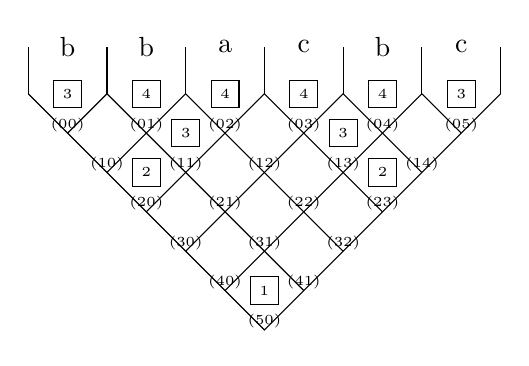
\begin{tikzpicture}[baseline]
			\newcommand{\myfontvars}[1]{
				\fontsize{4.9}{12}\selectfont{#1}
			}\newcommand{\myfontnumbering}[1]{
				\fontsize{2.5}{12}\selectfont{#1}
			}%Outer hull
			%Tip of the pyramid
			\coordinate (tip) at (3.0,-3.0);
			\foreach \i in {0,...,6} {
				\coordinate (\i) at (\i,0);
			}
			%Draw the left and right line of the pyramid pointing downwards
			\draw (0) -- (tip) -- (6);
			%Grid lines direction down-left to top-right
			\coordinate (dl1) at (0.5,-0.5);
			\coordinate (dl2) at (1.0,-1.0);
			\coordinate (dl3) at (1.5,-1.5);
			\coordinate (dl4) at (2.0,-2.0);
			\coordinate (dl5) at (2.5,-2.5);
			\draw (dl1) -- (1,0);
			\draw (dl2) -- (2,0);
			\draw (dl3) -- (3,0);
			\draw (dl4) -- (4,0);
			\draw (dl5) -- (5,0);
			%Grid lines direction down-right to top-left
			\coordinate (dr1) at (3.5,-2.5);
			\coordinate (dr2) at (4.0,-2.0);
			\coordinate (dr3) at (4.5,-1.5);
			\coordinate (dr4) at (5.0,-1.0);
			\coordinate (dr5) at (5.5,-0.5);
			\draw (dr1) -- (1,0);
			\draw (dr2) -- (2,0);
			\draw (dr3) -- (3,0);
			\draw (dr4) -- (4,0);
			\draw (dr5) -- (5,0);
			%Small lines at the top
			\coordinate (top0) at (0.0,0.0);
			\coordinate (top1) at (1.0,0.0);
			\coordinate (top2) at (2.0,0.0);
			\coordinate (top3) at (3.0,0.0);
			\coordinate (top4) at (4.0,0.0);
			\coordinate (top5) at (5.0,0.0);
			\coordinate (top6) at (6.0,0.0);
			\coordinate (topUpper0) at (0.0,0.6);
			\coordinate (topUpper1) at (1.0,0.6);
			\coordinate (topUpper2) at (2.0,0.6);
			\coordinate (topUpper3) at (3.0,0.6);
			\coordinate (topUpper4) at (4.0,0.6);
			\coordinate (topUpper5) at (5.0,0.6);
			\coordinate (topUpper6) at (6.0,0.6);
			\draw (top0) -- (topUpper0);
			\draw (top1) -- (topUpper1);
			\draw (top2) -- (topUpper2);
			\draw (top3) -- (topUpper3);
			\draw (top4) -- (topUpper4);
			\draw (top5) -- (topUpper5);
			\draw (top6) -- (topUpper6);
			%The string
			\coordinate (w0) at (0.5,0.6);
			\coordinate (w1) at (1.5,0.6);
			\coordinate (w2) at (2.5,0.6);
			\coordinate (w3) at (3.5,0.6);
			\coordinate (w4) at (4.5,0.6);
			\coordinate (w5) at (5.5,0.6);
			\node [] at (w0) {b};
			\node [] at (w1) {b};
			\node [] at (w2) {a};
			\node [] at (w3) {c};
			\node [] at (w4) {b};
			\node [] at (w5) {c};
			% Variables in the cells
			%cells00
			\coordinate (center00) at (0.5,0.0);
			\node [below=0.18cm] at (center00) {\myfontnumbering{$(00)$}};
			\node [] at (center00) [minimum height=0.25cm,minimum width=0.25cm,draw] {\tiny{3}};
			%cells01
			\coordinate (center01) at (1.5,0.0);
			\node [below=0.18cm] at (center01) {\myfontnumbering{$(01)$}};
			\node [] at (center01) [minimum height=0.25cm,minimum width=0.25cm,draw] {\tiny{4}};
			%cells02
			\coordinate (center02) at (2.5,0.0);
			\node [below=0.18cm] at (center02) {\myfontnumbering{$(02)$}};
			\node [] at (center02) [minimum height=0.25cm,minimum width=0.25cm,draw] {\tiny{4}};
			%cells03
			\coordinate (center03) at (3.5,0.0);
			\node [below=0.18cm] at (center03) {\myfontnumbering{$(03)$}};
			\node [] at (center03) [minimum height=0.25cm,minimum width=0.25cm,draw] {\tiny{4}};
			%cells04
			\coordinate (center04) at (4.5,0.0);
			\node [below=0.18cm] at (center04) {\myfontnumbering{$(04)$}};
			\node [] at (center04) [minimum height=0.25cm,minimum width=0.25cm,draw] {\tiny{4}};
			%cells05
			\coordinate (center05) at (5.5,0.0);
			\node [below=0.18cm] at (center05) {\myfontnumbering{$(05)$}};
			\node [] at (center05) [minimum height=0.25cm,minimum width=0.25cm,draw] {\tiny{3}};
			%cells10
			\coordinate (center10) at (1.0,-0.5);
			\node [below=0.18cm] at (center10) {\myfontnumbering{$(10)$}};
			%cells11
			\coordinate (center11) at (2.0,-0.5);
			\node [below=0.18cm] at (center11) {\myfontnumbering{$(11)$}};
			\node [] at (center11) [minimum height=0.25cm,minimum width=0.25cm,draw] {\tiny{3}};
			%cells12
			\coordinate (center12) at (3.0,-0.5);
			\node [below=0.18cm] at (center12) {\myfontnumbering{$(12)$}};
			%cells13
			\coordinate (center13) at (4.0,-0.5);
			\node [below=0.18cm] at (center13) {\myfontnumbering{$(13)$}};
			\node [] at (center13) [minimum height=0.25cm,minimum width=0.25cm,draw] {\tiny{3}};
			%cells14
			\coordinate (center14) at (5.0,-0.5);
			\node [below=0.18cm] at (center14) {\myfontnumbering{$(14)$}};
			%cells20
			\coordinate (center20) at (1.5,-1.0);
			\node [below=0.18cm] at (center20) {\myfontnumbering{$(20)$}};
			\node [] at (center20) [minimum height=0.25cm,minimum width=0.25cm,draw] {\tiny{2}};
			%cells21
			\coordinate (center21) at (2.5,-1.0);
			\node [below=0.18cm] at (center21) {\myfontnumbering{$(21)$}};
			%cells22
			\coordinate (center22) at (3.5,-1.0);
			\node [below=0.18cm] at (center22) {\myfontnumbering{$(22)$}};
			%cells23
			\coordinate (center23) at (4.5,-1.0);
			\node [below=0.18cm] at (center23) {\myfontnumbering{$(23)$}};
			\node [] at (center23) [minimum height=0.25cm,minimum width=0.25cm,draw] {\tiny{2}};
			%cells30
			\coordinate (center30) at (2.0,-1.5);
			\node [below=0.18cm] at (center30) {\myfontnumbering{$(30)$}};
			%cells31
			\coordinate (center31) at (3.0,-1.5);
			\node [below=0.18cm] at (center31) {\myfontnumbering{$(31)$}};
			%cells32
			\coordinate (center32) at (4.0,-1.5);
			\node [below=0.18cm] at (center32) {\myfontnumbering{$(32)$}};
			%cells40
			\coordinate (center40) at (2.5,-2.0);
			\node [below=0.18cm] at (center40) {\myfontnumbering{$(40)$}};
			%cells41
			\coordinate (center41) at (3.5,-2.0);
			\node [below=0.18cm] at (center41) {\myfontnumbering{$(41)$}};
			%cells50
			\coordinate (center50) at (3.0,-2.5);
			\node [below=0.18cm] at (center50) {\myfontnumbering{$(50)$}};
			\node [] at (center50) [minimum height=0.25cm,minimum width=0.25cm,draw] {\tiny{1}};
			\end{tikzpicture}
		}
		\resizebox{0.70\linewidth}{!}{
			
\begin{tikzpicture}[baseline]
			\tikzset{frontier/.style={distance from root=150pt}} %height of tree times 30pt
			\tikzset{edge from parent/.style= {
					draw,
					edge from parent path={(\tikzparentnode.south)	-- +(0,-8pt)-| (\tikzchildnode)}
				}
			}
			\Tree
			[.$Cell_{5,0}$
				[.$Cell_{2,0}$
					[.$Cell_{0,0}$ b ]
					[.$Cell_{1,1}$
						[.$Cell_{0,1}$ b ]
						[.$Cell_{0,2}$ a ]
					]
				]
			[.$Cell_{2,3}$
				[.$Cell_{1,3}$
					[.$Cell_{0,3}$ c ]
					[.$Cell_{0,4}$ b ]
				]
				[.$Cell_{0,5}$ c ]
			]
			]
			\end{tikzpicture}
		}
	\end{minipage}
		\label{treeStruct}
		\caption{Example derivation tree structure. Top: Shown in the pyramid, the numbers correspond to the depth in the tree. Down: Shown as a derivation tree.}
\end{figure}

\noindent As the name of the algorithms implies only after completely generating the structure of the derivation tree (splitting of the word in subwords) the rules are added to the grammar that help filling the cells occurring in the derivation tree.\\
Now every time before adding a new rule (Algorithm \ref{SplitThenFillRecursion} SplitThenFillRec Line \ref{splitThenFillB}) the already available information regarding the other rules is used to determine if a new rule is needed to fill this node of the derivation tree (Line \ref{empty} of Algorithm \ref{SplitThenFillRecursion} SplitThenFillRec).\\


\noindent
\frame{
	\begin{algorithm}[H] %or another one check
		\caption{SplitThenFill}
		\label{SplitThenFill}
		\SetAlgoLined
		\KwIn{Word $w \in \Sigma^{*}$}
		\KwOut{Set of productions $P$}
		$P = \emptyset$;~~\tcp{$P \subseteq V \times (V^{2} \cup \Sigma)$}
		$P = Distribute(\Sigma,\ V)$; \circled{A} \label{splitThenStepii}  \\		
		$Sol = (P_{Sol},~Cell_{i_{max},0})$;~~\tcp{$P_{Sol} \subseteq P~\wedge~ Cell_{i_{max},0} \in Pyramid$} \label{cell}
		$Sol = SplitThenFillRec(P,\ w,\ i_{max},\ 0)$\; \label{splitThenFillTreeStart}
		\Return $P_{Sol}$\;
		\footnotetext{
			\noindent Line \ref{splitThenStepii}: Fills the i=0 row of the pyramid.	
		}
	\end{algorithm}
}
\\
For this algorithm it is important to mention that while using \circled{B} (Line \ref{splitThenFillB} of Algorithm \ref{SplitThenFillRecursion}) a variable compound is added to at least one $lhse$. For every element of $vc \in VarComp$ (Line \ref{splitThenFillVc} of Algorithm \ref{SplitThenFillRecursion}) there exists at least one rule $lhse \rightarrow vc$.\\

\noindent
\frame{
	\begin{algorithm}[H] %or another one check
		\caption{SplitThenFillRec}
		\label{SplitThenFillRecursion}
		\SetAlgoLined
		\KwIn{$P_{in} \subseteq V \times (V^{2} \cup \Sigma),\ w \in \Sigma^{*},\ i,j \in \mathbb{N}$ }
		\KwOut{$(P,~Cell_{i,j})$}
		$P =  P_{in}$\;
		\If{$i=0$}{
			\Return $(P,\ Cell_{i,j})$\label{row0}\;
		}	
		$choose\ one\ m\ uniform\ randomly\ in\ [j+1,\ j+i]$\;
		$(P,\ Cell_l) = SplitThenFillRec(P,\ w,\ (m-j-1),\ j)$\label{left}\;
		$(P,\ Cell_r) = SplitThenFillRec(P,\ w,\ (j+i-m),\ m)$\label{right}\;
		$Pyramid = CYK(G,\ w)$\label{cyk}\;
		\If{$stopping\ criteria~met$~\circled{C}}{
			\Return $(P,\ Cell_{i,j})$\;
		}
		\If{$Cell_{i,j} = \emptyset$}{ \label{empty}
			$VarComp = uniform\ random\ subset\ from\ \{vc\ |\ v \in Cell_l\ \wedge $\\$~~~c \in Cell_r\} ~with~|VarComp| \geq 1$\; \label{splitThenFillVc}
			$P \cup Distribute(VarComp,\ V) $; \circled{B} \label{splitThenFillB}  \\
		}
		
		\Return $(P,\ Cell_{i,j})$\;
	\end{algorithm}
}
\clearpage
\noindent The same example tree structure as in Figure \ref{treeStruct} is used in the following example \textendash~each number represents the recursion depth of its subtree: 

\noindent
\begin{figure} [h]
	\begin{minipage}{6in}
		\centering
		\begin{tabular}{l}
			Grammar:\\
			$A \rightarrow a$\\
			$B \rightarrow b$\\ 
			$C \rightarrow c$\\
			$S \rightarrow $\\ 
		\end{tabular} 
		\resizebox{0.7\linewidth}{!}{
			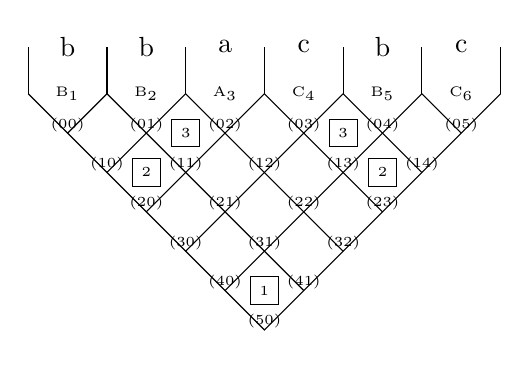
\begin{tikzpicture}[baseline]
			\newcommand{\myfontvars}[1]{
				\fontsize{4.9}{12}\selectfont{#1}
			}\newcommand{\myfontnumbering}[1]{
				\fontsize{2.5}{12}\selectfont{#1}
			}%Outer hull
			%Tip of the pyramid
			\coordinate (tip) at (3.0,-3.0);
			\foreach \i in {0,...,6} {
				\coordinate (\i) at (\i,0);
			}
			%Draw the left and right line of the pyramid pointing downwards
			\draw (0) -- (tip) -- (6);
			%Grid lines direction down-left to top-right
			\coordinate (dl1) at (0.5,-0.5);
			\coordinate (dl2) at (1.0,-1.0);
			\coordinate (dl3) at (1.5,-1.5);
			\coordinate (dl4) at (2.0,-2.0);
			\coordinate (dl5) at (2.5,-2.5);
			\draw (dl1) -- (1,0);
			\draw (dl2) -- (2,0);
			\draw (dl3) -- (3,0);
			\draw (dl4) -- (4,0);
			\draw (dl5) -- (5,0);
			%Grid lines direction down-right to top-left
			\coordinate (dr1) at (3.5,-2.5);
			\coordinate (dr2) at (4.0,-2.0);
			\coordinate (dr3) at (4.5,-1.5);
			\coordinate (dr4) at (5.0,-1.0);
			\coordinate (dr5) at (5.5,-0.5);
			\draw (dr1) -- (1,0);
			\draw (dr2) -- (2,0);
			\draw (dr3) -- (3,0);
			\draw (dr4) -- (4,0);
			\draw (dr5) -- (5,0);
			%Small lines at the top
			\coordinate (top0) at (0.0,0.0);
			\coordinate (top1) at (1.0,0.0);
			\coordinate (top2) at (2.0,0.0);
			\coordinate (top3) at (3.0,0.0);
			\coordinate (top4) at (4.0,0.0);
			\coordinate (top5) at (5.0,0.0);
			\coordinate (top6) at (6.0,0.0);
			\coordinate (topUpper0) at (0.0,0.6);
			\coordinate (topUpper1) at (1.0,0.6);
			\coordinate (topUpper2) at (2.0,0.6);
			\coordinate (topUpper3) at (3.0,0.6);
			\coordinate (topUpper4) at (4.0,0.6);
			\coordinate (topUpper5) at (5.0,0.6);
			\coordinate (topUpper6) at (6.0,0.6);
			\draw (top0) -- (topUpper0);
			\draw (top1) -- (topUpper1);
			\draw (top2) -- (topUpper2);
			\draw (top3) -- (topUpper3);
			\draw (top4) -- (topUpper4);
			\draw (top5) -- (topUpper5);
			\draw (top6) -- (topUpper6);
			%The string
			\coordinate (w0) at (0.5,0.6);
			\coordinate (w1) at (1.5,0.6);
			\coordinate (w2) at (2.5,0.6);
			\coordinate (w3) at (3.5,0.6);
			\coordinate (w4) at (4.5,0.6);
			\coordinate (w5) at (5.5,0.6);
			\node [] at (w0) {b};
			\node [] at (w1) {b};
			\node [] at (w2) {a};
			\node [] at (w3) {c};
			\node [] at (w4) {b};
			\node [] at (w5) {c};
			% Variables in the cells
			%cells00
			\coordinate (center00) at (0.5,0.0);
			\node [below=0.18cm] at (center00) {\myfontnumbering{$(00)$}};
			\node [] at (center00) {\myfontvars{B$_{1}$}};
			%cells01
			\coordinate (center01) at (1.5,0.0);
			\node [below=0.18cm] at (center01) {\myfontnumbering{$(01)$}};
			\node [] at (center01) {\myfontvars{B$_{2}$}};
			%cells02
			\coordinate (center02) at (2.5,0.0);
			\node [below=0.18cm] at (center02) {\myfontnumbering{$(02)$}};
			\node [] at (center02) {\myfontvars{A$_{3}$}};
			%cells03
			\coordinate (center03) at (3.5,0.0);
			\node [below=0.18cm] at (center03) {\myfontnumbering{$(03)$}};
			\node [] at (center03) {\myfontvars{C$_{4}$}};
			%cells04
			\coordinate (center04) at (4.5,0.0);
			\node [below=0.18cm] at (center04) {\myfontnumbering{$(04)$}};
			\node [] at (center04) {\myfontvars{B$_{5}$}};
			%cells05
			\coordinate (center05) at (5.5,0.0);
			\node [below=0.18cm] at (center05) {\myfontnumbering{$(05)$}};
			\node [] at (center05) {\myfontvars{C$_{6}$}};
			%cells10
			\coordinate (center10) at (1.0,-0.5);
			\node [below=0.18cm] at (center10) {\myfontnumbering{$(10)$}};
			%cells11
			\coordinate (center11) at (2.0,-0.5);
			\node [below=0.18cm] at (center11) {\myfontnumbering{$(11)$}};
			\node [] at (center11) [minimum height=0.25cm,minimum width=0.25cm,draw] {\tiny{3}};
			%cells12
			\coordinate (center12) at (3.0,-0.5);
			\node [below=0.18cm] at (center12) {\myfontnumbering{$(12)$}};
			%cells13
			\coordinate (center13) at (4.0,-0.5);
			\node [below=0.18cm] at (center13) {\myfontnumbering{$(13)$}};
			\node [] at (center13) [minimum height=0.25cm,minimum width=0.25cm,draw] {\tiny{3}};
			%cells14
			\coordinate (center14) at (5.0,-0.5);
			\node [below=0.18cm] at (center14) {\myfontnumbering{$(14)$}};
			%cells20
			\coordinate (center20) at (1.5,-1.0);
			\node [below=0.18cm] at (center20) {\myfontnumbering{$(20)$}};
			\node [] at (center20) [minimum height=0.25cm,minimum width=0.25cm,draw] {\tiny{2}};
			%cells21
			\coordinate (center21) at (2.5,-1.0);
			\node [below=0.18cm] at (center21) {\myfontnumbering{$(21)$}};
			%cells22
			\coordinate (center22) at (3.5,-1.0);
			\node [below=0.18cm] at (center22) {\myfontnumbering{$(22)$}};
			%cells23
			\coordinate (center23) at (4.5,-1.0);
			\node [below=0.18cm] at (center23) {\myfontnumbering{$(23)$}};
			\node [] at (center23) [minimum height=0.25cm,minimum width=0.25cm,draw] {\tiny{2}};
			%cells30
			\coordinate (center30) at (2.0,-1.5);
			\node [below=0.18cm] at (center30) {\myfontnumbering{$(30)$}};
			%cells31
			\coordinate (center31) at (3.0,-1.5);
			\node [below=0.18cm] at (center31) {\myfontnumbering{$(31)$}};
			%cells32
			\coordinate (center32) at (4.0,-1.5);
			\node [below=0.18cm] at (center32) {\myfontnumbering{$(32)$}};
			%cells40
			\coordinate (center40) at (2.5,-2.0);
			\node [below=0.18cm] at (center40) {\myfontnumbering{$(40)$}};
			%cells41
			\coordinate (center41) at (3.5,-2.0);
			\node [below=0.18cm] at (center41) {\myfontnumbering{$(41)$}};
			%cells50
			\coordinate (center50) at (3.0,-2.5);
			\node [below=0.18cm] at (center50) {\myfontnumbering{$(50)$}};
			\node [] at (center50) [minimum height=0.25cm,minimum width=0.25cm,draw] {\tiny{1}};
			\end{tikzpicture}
		}
	\end{minipage}
	\caption{Illustration of Algorithm \ref{SplitThenFill} SplitThenFill part 1 after adding $A \rightarrow a$, $B \rightarrow b$ and $C \rightarrow c$.}
	\label{IllustrationAlgorithmSplitThenFillPart1}
\end{figure}

\noindent After adding the terminals to the grammar (Line \ref{splitThenStepii} in Algorithm \ref{SplitThenFill} SplitThenFill) now the recursion step at $Cell_{1,1}$ is taken on. Now $Cell_l=\{B_2\}$ and $Cell_r=\{A_3\}$ and therefore $VarComp=\{BA\}$. Adding the rule $S \rightarrow BA$ leads to the following $Pyramid$: 

\noindent
\begin{figure} [h]
	\begin{minipage}{6in}
		\centering
		\begin{tabular}{l}
			Grammar:\\
			$A \rightarrow a$\\
			$B \rightarrow b$\\ 
			$C \rightarrow c$\\
			$S \rightarrow BA$\\ 
		\end{tabular} 
		\resizebox{0.7\linewidth}{!}{
			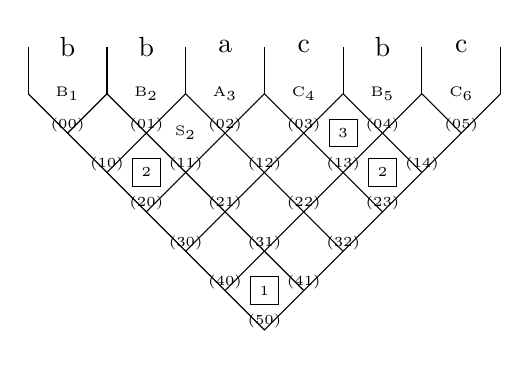
\begin{tikzpicture}[baseline]
			\newcommand{\myfontvars}[1]{
				\fontsize{4.9}{12}\selectfont{#1}
			}\newcommand{\myfontnumbering}[1]{
				\fontsize{2.5}{12}\selectfont{#1}
			}%Outer hull
			%Tip of the pyramid
			\coordinate (tip) at (3.0,-3.0);
			\foreach \i in {0,...,6} {
				\coordinate (\i) at (\i,0);
			}
			%Draw the left and right line of the pyramid pointing downwards
			\draw (0) -- (tip) -- (6);
			%Grid lines direction down-left to top-right
			\coordinate (dl1) at (0.5,-0.5);
			\coordinate (dl2) at (1.0,-1.0);
			\coordinate (dl3) at (1.5,-1.5);
			\coordinate (dl4) at (2.0,-2.0);
			\coordinate (dl5) at (2.5,-2.5);
			\draw (dl1) -- (1,0);
			\draw (dl2) -- (2,0);
			\draw (dl3) -- (3,0);
			\draw (dl4) -- (4,0);
			\draw (dl5) -- (5,0);
			%Grid lines direction down-right to top-left
			\coordinate (dr1) at (3.5,-2.5);
			\coordinate (dr2) at (4.0,-2.0);
			\coordinate (dr3) at (4.5,-1.5);
			\coordinate (dr4) at (5.0,-1.0);
			\coordinate (dr5) at (5.5,-0.5);
			\draw (dr1) -- (1,0);
			\draw (dr2) -- (2,0);
			\draw (dr3) -- (3,0);
			\draw (dr4) -- (4,0);
			\draw (dr5) -- (5,0);
			%Small lines at the top
			\coordinate (top0) at (0.0,0.0);
			\coordinate (top1) at (1.0,0.0);
			\coordinate (top2) at (2.0,0.0);
			\coordinate (top3) at (3.0,0.0);
			\coordinate (top4) at (4.0,0.0);
			\coordinate (top5) at (5.0,0.0);
			\coordinate (top6) at (6.0,0.0);
			\coordinate (topUpper0) at (0.0,0.6);
			\coordinate (topUpper1) at (1.0,0.6);
			\coordinate (topUpper2) at (2.0,0.6);
			\coordinate (topUpper3) at (3.0,0.6);
			\coordinate (topUpper4) at (4.0,0.6);
			\coordinate (topUpper5) at (5.0,0.6);
			\coordinate (topUpper6) at (6.0,0.6);
			\draw (top0) -- (topUpper0);
			\draw (top1) -- (topUpper1);
			\draw (top2) -- (topUpper2);
			\draw (top3) -- (topUpper3);
			\draw (top4) -- (topUpper4);
			\draw (top5) -- (topUpper5);
			\draw (top6) -- (topUpper6);
			%The string
			\coordinate (w0) at (0.5,0.6);
			\coordinate (w1) at (1.5,0.6);
			\coordinate (w2) at (2.5,0.6);
			\coordinate (w3) at (3.5,0.6);
			\coordinate (w4) at (4.5,0.6);
			\coordinate (w5) at (5.5,0.6);
			\node [] at (w0) {b};
			\node [] at (w1) {b};
			\node [] at (w2) {a};
			\node [] at (w3) {c};
			\node [] at (w4) {b};
			\node [] at (w5) {c};
			% Variables in the cells
			%cells00
			\coordinate (center00) at (0.5,0.0);
			\node [below=0.18cm] at (center00) {\myfontnumbering{$(00)$}};
			\node [] at (center00) {\myfontvars{B$_{1}$}};
			%cells01
			\coordinate (center01) at (1.5,0.0);
			\node [below=0.18cm] at (center01) {\myfontnumbering{$(01)$}};
			\node [] at (center01) {\myfontvars{B$_{2}$}};
			%cells02
			\coordinate (center02) at (2.5,0.0);
			\node [below=0.18cm] at (center02) {\myfontnumbering{$(02)$}};
			\node [] at (center02) {\myfontvars{A$_{3}$}};
			%cells03
			\coordinate (center03) at (3.5,0.0);
			\node [below=0.18cm] at (center03) {\myfontnumbering{$(03)$}};
			\node [] at (center03) {\myfontvars{C$_{4}$}};
			%cells04
			\coordinate (center04) at (4.5,0.0);
			\node [below=0.18cm] at (center04) {\myfontnumbering{$(04)$}};
			\node [] at (center04) {\myfontvars{B$_{5}$}};
			%cells05
			\coordinate (center05) at (5.5,0.0);
			\node [below=0.18cm] at (center05) {\myfontnumbering{$(05)$}};
			\node [] at (center05) {\myfontvars{C$_{6}$}};
			%cells10
			\coordinate (center10) at (1.0,-0.5);
			\node [below=0.18cm] at (center10) {\myfontnumbering{$(10)$}};
			%cells11
			\coordinate (center11) at (2.0,-0.5);
			\node [below=0.18cm] at (center11) {\myfontnumbering{$(11)$}};
			\node [] at (center11) {\myfontvars{S$_{2}$}};
			%cells12
			\coordinate (center12) at (3.0,-0.5);
			\node [below=0.18cm] at (center12) {\myfontnumbering{$(12)$}};
			%cells13
			\coordinate (center13) at (4.0,-0.5);
			\node [below=0.18cm] at (center13) {\myfontnumbering{$(13)$}};
			\node [] at (center13) [minimum height=0.25cm,minimum width=0.25cm,draw] {\tiny{3}};
			%cells14
			\coordinate (center14) at (5.0,-0.5);
			\node [below=0.18cm] at (center14) {\myfontnumbering{$(14)$}};
			%cells20
			\coordinate (center20) at (1.5,-1.0);
			\node [below=0.18cm] at (center20) {\myfontnumbering{$(20)$}};
			\node [] at (center20) [minimum height=0.25cm,minimum width=0.25cm,draw] {\tiny{2}};
			%cells21
			\coordinate (center21) at (2.5,-1.0);
			\node [below=0.18cm] at (center21) {\myfontnumbering{$(21)$}};
			%cells22
			\coordinate (center22) at (3.5,-1.0);
			\node [below=0.18cm] at (center22) {\myfontnumbering{$(22)$}};
			%cells23
			\coordinate (center23) at (4.5,-1.0);
			\node [below=0.18cm] at (center23) {\myfontnumbering{$(23)$}};
			\node [] at (center23) [minimum height=0.25cm,minimum width=0.25cm,draw] {\tiny{2}};
			%cells30
			\coordinate (center30) at (2.0,-1.5);
			\node [below=0.18cm] at (center30) {\myfontnumbering{$(30)$}};
			%cells31
			\coordinate (center31) at (3.0,-1.5);
			\node [below=0.18cm] at (center31) {\myfontnumbering{$(31)$}};
			%cells32
			\coordinate (center32) at (4.0,-1.5);
			\node [below=0.18cm] at (center32) {\myfontnumbering{$(32)$}};
			%cells40
			\coordinate (center40) at (2.5,-2.0);
			\node [below=0.18cm] at (center40) {\myfontnumbering{$(40)$}};
			%cells41
			\coordinate (center41) at (3.5,-2.0);
			\node [below=0.18cm] at (center41) {\myfontnumbering{$(41)$}};
			%cells50
			\coordinate (center50) at (3.0,-2.5);
			\node [below=0.18cm] at (center50) {\myfontnumbering{$(50)$}};
			\node [] at (center50) [minimum height=0.25cm,minimum width=0.25cm,draw] {\tiny{1}};
			\end{tikzpicture}
		}
	\end{minipage}
	\caption{Illustration of Algorithm \ref{SplitThenFill} SplitThenFill part 2 after adding $S\rightarrow BA$.}
	\label{IllustrationAlgorithmSplitThenFillPart2}
\end{figure}\\
\clearpage
\noindent The next recursion step happens in $Cell_{2,0}$. Now $Cell_l=\{B_1\}$ and $Cell_r=\{S_2\}$. Analogously the rule $A\rightarrow BS$ is added to the grammar:

\noindent
\begin{figure} [h]
	\begin{minipage}{6in}
		\centering
		\begin{tabular}{l}
			Grammar:\\
			$A \rightarrow BS~|~a$\\
			$B \rightarrow b$\\ 
			$C \rightarrow c$\\
			$S \rightarrow BA$\\ 
		\end{tabular} 
		\resizebox{0.7\linewidth}{!}{
			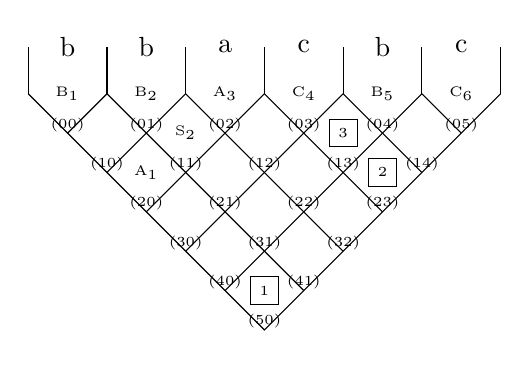
\begin{tikzpicture}[baseline]
			\newcommand{\myfontvars}[1]{
				\fontsize{4.9}{12}\selectfont{#1}
			}\newcommand{\myfontnumbering}[1]{
				\fontsize{2.5}{12}\selectfont{#1}
			}%Outer hull
			%Tip of the pyramid
			\coordinate (tip) at (3.0,-3.0);
			\foreach \i in {0,...,6} {
				\coordinate (\i) at (\i,0);
			}
			%Draw the left and right line of the pyramid pointing downwards
			\draw (0) -- (tip) -- (6);
			%Grid lines direction down-left to top-right
			\coordinate (dl1) at (0.5,-0.5);
			\coordinate (dl2) at (1.0,-1.0);
			\coordinate (dl3) at (1.5,-1.5);
			\coordinate (dl4) at (2.0,-2.0);
			\coordinate (dl5) at (2.5,-2.5);
			\draw (dl1) -- (1,0);
			\draw (dl2) -- (2,0);
			\draw (dl3) -- (3,0);
			\draw (dl4) -- (4,0);
			\draw (dl5) -- (5,0);
			%Grid lines direction down-right to top-left
			\coordinate (dr1) at (3.5,-2.5);
			\coordinate (dr2) at (4.0,-2.0);
			\coordinate (dr3) at (4.5,-1.5);
			\coordinate (dr4) at (5.0,-1.0);
			\coordinate (dr5) at (5.5,-0.5);
			\draw (dr1) -- (1,0);
			\draw (dr2) -- (2,0);
			\draw (dr3) -- (3,0);
			\draw (dr4) -- (4,0);
			\draw (dr5) -- (5,0);
			%Small lines at the top
			\coordinate (top0) at (0.0,0.0);
			\coordinate (top1) at (1.0,0.0);
			\coordinate (top2) at (2.0,0.0);
			\coordinate (top3) at (3.0,0.0);
			\coordinate (top4) at (4.0,0.0);
			\coordinate (top5) at (5.0,0.0);
			\coordinate (top6) at (6.0,0.0);
			\coordinate (topUpper0) at (0.0,0.6);
			\coordinate (topUpper1) at (1.0,0.6);
			\coordinate (topUpper2) at (2.0,0.6);
			\coordinate (topUpper3) at (3.0,0.6);
			\coordinate (topUpper4) at (4.0,0.6);
			\coordinate (topUpper5) at (5.0,0.6);
			\coordinate (topUpper6) at (6.0,0.6);
			\draw (top0) -- (topUpper0);
			\draw (top1) -- (topUpper1);
			\draw (top2) -- (topUpper2);
			\draw (top3) -- (topUpper3);
			\draw (top4) -- (topUpper4);
			\draw (top5) -- (topUpper5);
			\draw (top6) -- (topUpper6);
			%The string
			\coordinate (w0) at (0.5,0.6);
			\coordinate (w1) at (1.5,0.6);
			\coordinate (w2) at (2.5,0.6);
			\coordinate (w3) at (3.5,0.6);
			\coordinate (w4) at (4.5,0.6);
			\coordinate (w5) at (5.5,0.6);
			\node [] at (w0) {b};
			\node [] at (w1) {b};
			\node [] at (w2) {a};
			\node [] at (w3) {c};
			\node [] at (w4) {b};
			\node [] at (w5) {c};
			% Variables in the cells
			%cells00
			\coordinate (center00) at (0.5,0.0);
			\node [below=0.18cm] at (center00) {\myfontnumbering{$(00)$}};
			\node [] at (center00) {\myfontvars{B$_{1}$}};
			%cells01
			\coordinate (center01) at (1.5,0.0);
			\node [below=0.18cm] at (center01) {\myfontnumbering{$(01)$}};
			\node [] at (center01) {\myfontvars{B$_{2}$}};
			%cells02
			\coordinate (center02) at (2.5,0.0);
			\node [below=0.18cm] at (center02) {\myfontnumbering{$(02)$}};
			\node [] at (center02) {\myfontvars{A$_{3}$}};
			%cells03
			\coordinate (center03) at (3.5,0.0);
			\node [below=0.18cm] at (center03) {\myfontnumbering{$(03)$}};
			\node [] at (center03) {\myfontvars{C$_{4}$}};
			%cells04
			\coordinate (center04) at (4.5,0.0);
			\node [below=0.18cm] at (center04) {\myfontnumbering{$(04)$}};
			\node [] at (center04) {\myfontvars{B$_{5}$}};
			%cells05
			\coordinate (center05) at (5.5,0.0);
			\node [below=0.18cm] at (center05) {\myfontnumbering{$(05)$}};
			\node [] at (center05) {\myfontvars{C$_{6}$}};
			%cells10
			\coordinate (center10) at (1.0,-0.5);
			\node [below=0.18cm] at (center10) {\myfontnumbering{$(10)$}};
			%cells11
			\coordinate (center11) at (2.0,-0.5);
			\node [below=0.18cm] at (center11) {\myfontnumbering{$(11)$}};
			\node [] at (center11) {\myfontvars{S$_{2}$}};
			%cells12
			\coordinate (center12) at (3.0,-0.5);
			\node [below=0.18cm] at (center12) {\myfontnumbering{$(12)$}};
			%cells13
			\coordinate (center13) at (4.0,-0.5);
			\node [below=0.18cm] at (center13) {\myfontnumbering{$(13)$}};
			\node [] at (center13) [minimum height=0.25cm,minimum width=0.25cm,draw] {\tiny{3}};
			%cells14
			\coordinate (center14) at (5.0,-0.5);
			\node [below=0.18cm] at (center14) {\myfontnumbering{$(14)$}};
			%cells20
			\coordinate (center20) at (1.5,-1.0);
			\node [below=0.18cm] at (center20) {\myfontnumbering{$(20)$}};
			\node [] at (center20) {\myfontvars{A$_{1}$}};
			%cells21
			\coordinate (center21) at (2.5,-1.0);
			\node [below=0.18cm] at (center21) {\myfontnumbering{$(21)$}};
			%cells22
			\coordinate (center22) at (3.5,-1.0);
			\node [below=0.18cm] at (center22) {\myfontnumbering{$(22)$}};
			%cells23
			\coordinate (center23) at (4.5,-1.0);
			\node [below=0.18cm] at (center23) {\myfontnumbering{$(23)$}};
			\node [] at (center23) [minimum height=0.25cm,minimum width=0.25cm,draw] {\tiny{2}};
			%cells30
			\coordinate (center30) at (2.0,-1.5);
			\node [below=0.18cm] at (center30) {\myfontnumbering{$(30)$}};
			%cells31
			\coordinate (center31) at (3.0,-1.5);
			\node [below=0.18cm] at (center31) {\myfontnumbering{$(31)$}};
			%cells32
			\coordinate (center32) at (4.0,-1.5);
			\node [below=0.18cm] at (center32) {\myfontnumbering{$(32)$}};
			%cells40
			\coordinate (center40) at (2.5,-2.0);
			\node [below=0.18cm] at (center40) {\myfontnumbering{$(40)$}};
			%cells41
			\coordinate (center41) at (3.5,-2.0);
			\node [below=0.18cm] at (center41) {\myfontnumbering{$(41)$}};
			%cells50
			\coordinate (center50) at (3.0,-2.5);
			\node [below=0.18cm] at (center50) {\myfontnumbering{$(50)$}};
			\node [] at (center50) [minimum height=0.25cm,minimum width=0.25cm,draw] {\tiny{1}};
			\end{tikzpicture}
		}
	\end{minipage}
	\caption{Illustration of Algorithm \ref{SplitThenFill} SplitThenFill part 3 after adding the rule $A\rightarrow BS$.}
	\label{IllustrationAlgorithmSplitThenFillPart3}
\end{figure}\\
The next two analogous steps are described in Figure \ref{IllustrationAlgorithmSplitThenFillPart4} and in Figure \ref{IllustrationAlgorithmSplitThenFillPart5}. \\
\noindent
\begin{figure} [h]
	\begin{minipage}{6in}
		\centering
		\begin{tabular}{l}
			Grammar:\\
			$A \rightarrow BS~|~a$\\
			$B \rightarrow CB~|~b$\\ 
			$C \rightarrow c$\\
			$S \rightarrow BA$\\ 
		\end{tabular} 
		\resizebox{0.7\linewidth}{!}{
			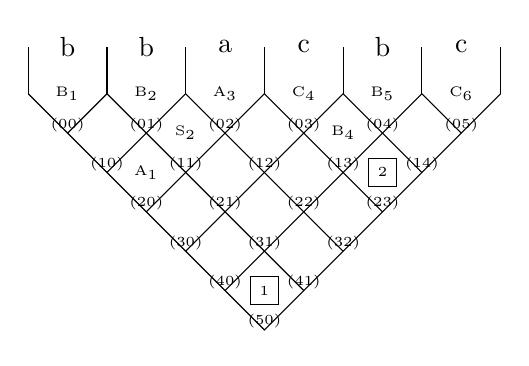
\begin{tikzpicture}[baseline]
			\newcommand{\myfontvars}[1]{
				\fontsize{4.9}{12}\selectfont{#1}
			}\newcommand{\myfontnumbering}[1]{
				\fontsize{2.5}{12}\selectfont{#1}
			}%Outer hull
			%Tip of the pyramid
			\coordinate (tip) at (3.0,-3.0);
			\foreach \i in {0,...,6} {
				\coordinate (\i) at (\i,0);
			}
			%Draw the left and right line of the pyramid pointing downwards
			\draw (0) -- (tip) -- (6);
			%Grid lines direction down-left to top-right
			\coordinate (dl1) at (0.5,-0.5);
			\coordinate (dl2) at (1.0,-1.0);
			\coordinate (dl3) at (1.5,-1.5);
			\coordinate (dl4) at (2.0,-2.0);
			\coordinate (dl5) at (2.5,-2.5);
			\draw (dl1) -- (1,0);
			\draw (dl2) -- (2,0);
			\draw (dl3) -- (3,0);
			\draw (dl4) -- (4,0);
			\draw (dl5) -- (5,0);
			%Grid lines direction down-right to top-left
			\coordinate (dr1) at (3.5,-2.5);
			\coordinate (dr2) at (4.0,-2.0);
			\coordinate (dr3) at (4.5,-1.5);
			\coordinate (dr4) at (5.0,-1.0);
			\coordinate (dr5) at (5.5,-0.5);
			\draw (dr1) -- (1,0);
			\draw (dr2) -- (2,0);
			\draw (dr3) -- (3,0);
			\draw (dr4) -- (4,0);
			\draw (dr5) -- (5,0);
			%Small lines at the top
			\coordinate (top0) at (0.0,0.0);
			\coordinate (top1) at (1.0,0.0);
			\coordinate (top2) at (2.0,0.0);
			\coordinate (top3) at (3.0,0.0);
			\coordinate (top4) at (4.0,0.0);
			\coordinate (top5) at (5.0,0.0);
			\coordinate (top6) at (6.0,0.0);
			\coordinate (topUpper0) at (0.0,0.6);
			\coordinate (topUpper1) at (1.0,0.6);
			\coordinate (topUpper2) at (2.0,0.6);
			\coordinate (topUpper3) at (3.0,0.6);
			\coordinate (topUpper4) at (4.0,0.6);
			\coordinate (topUpper5) at (5.0,0.6);
			\coordinate (topUpper6) at (6.0,0.6);
			\draw (top0) -- (topUpper0);
			\draw (top1) -- (topUpper1);
			\draw (top2) -- (topUpper2);
			\draw (top3) -- (topUpper3);
			\draw (top4) -- (topUpper4);
			\draw (top5) -- (topUpper5);
			\draw (top6) -- (topUpper6);
			%The string
			\coordinate (w0) at (0.5,0.6);
			\coordinate (w1) at (1.5,0.6);
			\coordinate (w2) at (2.5,0.6);
			\coordinate (w3) at (3.5,0.6);
			\coordinate (w4) at (4.5,0.6);
			\coordinate (w5) at (5.5,0.6);
			\node [] at (w0) {b};
			\node [] at (w1) {b};
			\node [] at (w2) {a};
			\node [] at (w3) {c};
			\node [] at (w4) {b};
			\node [] at (w5) {c};
			% Variables in the cells
			%cells00
			\coordinate (center00) at (0.5,0.0);
			\node [below=0.18cm] at (center00) {\myfontnumbering{$(00)$}};
			\node [] at (center00) {\myfontvars{B$_{1}$}};
			%cells01
			\coordinate (center01) at (1.5,0.0);
			\node [below=0.18cm] at (center01) {\myfontnumbering{$(01)$}};
			\node [] at (center01) {\myfontvars{B$_{2}$}};
			%cells02
			\coordinate (center02) at (2.5,0.0);
			\node [below=0.18cm] at (center02) {\myfontnumbering{$(02)$}};
			\node [] at (center02) {\myfontvars{A$_{3}$}};
			%cells03
			\coordinate (center03) at (3.5,0.0);
			\node [below=0.18cm] at (center03) {\myfontnumbering{$(03)$}};
			\node [] at (center03) {\myfontvars{C$_{4}$}};
			%cells04
			\coordinate (center04) at (4.5,0.0);
			\node [below=0.18cm] at (center04) {\myfontnumbering{$(04)$}};
			\node [] at (center04) {\myfontvars{B$_{5}$}};
			%cells05
			\coordinate (center05) at (5.5,0.0);
			\node [below=0.18cm] at (center05) {\myfontnumbering{$(05)$}};
			\node [] at (center05) {\myfontvars{C$_{6}$}};
			%cells10
			\coordinate (center10) at (1.0,-0.5);
			\node [below=0.18cm] at (center10) {\myfontnumbering{$(10)$}};
			%cells11
			\coordinate (center11) at (2.0,-0.5);
			\node [below=0.18cm] at (center11) {\myfontnumbering{$(11)$}};
			\node [] at (center11) {\myfontvars{S$_{2}$}};
			%cells12
			\coordinate (center12) at (3.0,-0.5);
			\node [below=0.18cm] at (center12) {\myfontnumbering{$(12)$}};
			%cells13
			\coordinate (center13) at (4.0,-0.5);
			\node [below=0.18cm] at (center13) {\myfontnumbering{$(13)$}};
			\node [] at (center13) {\myfontvars{B$_{4}$}};
			%cells14
			\coordinate (center14) at (5.0,-0.5);
			\node [below=0.18cm] at (center14) {\myfontnumbering{$(14)$}};
			%cells20
			\coordinate (center20) at (1.5,-1.0);
			\node [below=0.18cm] at (center20) {\myfontnumbering{$(20)$}};
			\node [] at (center20) {\myfontvars{A$_{1}$}};
			%cells21
			\coordinate (center21) at (2.5,-1.0);
			\node [below=0.18cm] at (center21) {\myfontnumbering{$(21)$}};
			%cells22
			\coordinate (center22) at (3.5,-1.0);
			\node [below=0.18cm] at (center22) {\myfontnumbering{$(22)$}};
			%cells23
			\coordinate (center23) at (4.5,-1.0);
			\node [below=0.18cm] at (center23) {\myfontnumbering{$(23)$}};
			\node [] at (center23) [minimum height=0.25cm,minimum width=0.25cm,draw] {\tiny{2}};
			%cells30
			\coordinate (center30) at (2.0,-1.5);
			\node [below=0.18cm] at (center30) {\myfontnumbering{$(30)$}};
			%cells31
			\coordinate (center31) at (3.0,-1.5);
			\node [below=0.18cm] at (center31) {\myfontnumbering{$(31)$}};
			%cells32
			\coordinate (center32) at (4.0,-1.5);
			\node [below=0.18cm] at (center32) {\myfontnumbering{$(32)$}};
			%cells40
			\coordinate (center40) at (2.5,-2.0);
			\node [below=0.18cm] at (center40) {\myfontnumbering{$(40)$}};
			%cells41
			\coordinate (center41) at (3.5,-2.0);
			\node [below=0.18cm] at (center41) {\myfontnumbering{$(41)$}};
			%cells50
			\coordinate (center50) at (3.0,-2.5);
			\node [below=0.18cm] at (center50) {\myfontnumbering{$(50)$}};
			\node [] at (center50) [minimum height=0.25cm,minimum width=0.25cm,draw] {\tiny{1}};
			\end{tikzpicture}
		}
	\end{minipage}
	\caption{Illustration of Algorithm \ref{SplitThenFill} SplitThenFill part 4. The recursion step in $Cell_{1,3}$ is  resolved by adding the rule $B\rightarrow CB$.}
	\label{IllustrationAlgorithmSplitThenFillPart4}
\end{figure}
\clearpage
\noindent
\begin{figure} [h]
	\begin{minipage}{6in}
		\centering
		\begin{tabular}{l}
			Grammar:\\
			$A \rightarrow BS~|~a$\\
			$B \rightarrow CB~|~b$\\ 
			$C \rightarrow BC~|~c$\\
			$S \rightarrow BA$\\ 
		\end{tabular} 
		\resizebox{0.7\linewidth}{!}{
			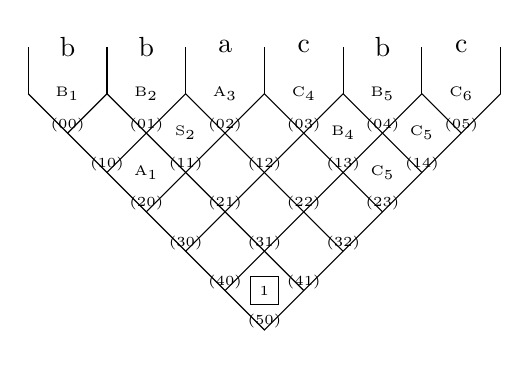
\begin{tikzpicture}[baseline]
			\newcommand{\myfontvars}[1]{
				\fontsize{4.9}{12}\selectfont{#1}
			}\newcommand{\myfontnumbering}[1]{
				\fontsize{2.5}{12}\selectfont{#1}
			}%Outer hull
			%Tip of the pyramid
			\coordinate (tip) at (3.0,-3.0);
			\foreach \i in {0,...,6} {
				\coordinate (\i) at (\i,0);
			}
			%Draw the left and right line of the pyramid pointing downwards
			\draw (0) -- (tip) -- (6);
			%Grid lines direction down-left to top-right
			\coordinate (dl1) at (0.5,-0.5);
			\coordinate (dl2) at (1.0,-1.0);
			\coordinate (dl3) at (1.5,-1.5);
			\coordinate (dl4) at (2.0,-2.0);
			\coordinate (dl5) at (2.5,-2.5);
			\draw (dl1) -- (1,0);
			\draw (dl2) -- (2,0);
			\draw (dl3) -- (3,0);
			\draw (dl4) -- (4,0);
			\draw (dl5) -- (5,0);
			%Grid lines direction down-right to top-left
			\coordinate (dr1) at (3.5,-2.5);
			\coordinate (dr2) at (4.0,-2.0);
			\coordinate (dr3) at (4.5,-1.5);
			\coordinate (dr4) at (5.0,-1.0);
			\coordinate (dr5) at (5.5,-0.5);
			\draw (dr1) -- (1,0);
			\draw (dr2) -- (2,0);
			\draw (dr3) -- (3,0);
			\draw (dr4) -- (4,0);
			\draw (dr5) -- (5,0);
			%Small lines at the top
			\coordinate (top0) at (0.0,0.0);
			\coordinate (top1) at (1.0,0.0);
			\coordinate (top2) at (2.0,0.0);
			\coordinate (top3) at (3.0,0.0);
			\coordinate (top4) at (4.0,0.0);
			\coordinate (top5) at (5.0,0.0);
			\coordinate (top6) at (6.0,0.0);
			\coordinate (topUpper0) at (0.0,0.6);
			\coordinate (topUpper1) at (1.0,0.6);
			\coordinate (topUpper2) at (2.0,0.6);
			\coordinate (topUpper3) at (3.0,0.6);
			\coordinate (topUpper4) at (4.0,0.6);
			\coordinate (topUpper5) at (5.0,0.6);
			\coordinate (topUpper6) at (6.0,0.6);
			\draw (top0) -- (topUpper0);
			\draw (top1) -- (topUpper1);
			\draw (top2) -- (topUpper2);
			\draw (top3) -- (topUpper3);
			\draw (top4) -- (topUpper4);
			\draw (top5) -- (topUpper5);
			\draw (top6) -- (topUpper6);
			%The string
			\coordinate (w0) at (0.5,0.6);
			\coordinate (w1) at (1.5,0.6);
			\coordinate (w2) at (2.5,0.6);
			\coordinate (w3) at (3.5,0.6);
			\coordinate (w4) at (4.5,0.6);
			\coordinate (w5) at (5.5,0.6);
			\node [] at (w0) {b};
			\node [] at (w1) {b};
			\node [] at (w2) {a};
			\node [] at (w3) {c};
			\node [] at (w4) {b};
			\node [] at (w5) {c};
			% Variables in the cells
			%cells00
			\coordinate (center00) at (0.5,0.0);
			\node [below=0.18cm] at (center00) {\myfontnumbering{$(00)$}};
			\node [] at (center00) {\myfontvars{B$_{1}$}};
			%cells01
			\coordinate (center01) at (1.5,0.0);
			\node [below=0.18cm] at (center01) {\myfontnumbering{$(01)$}};
			\node [] at (center01) {\myfontvars{B$_{2}$}};
			%cells02
			\coordinate (center02) at (2.5,0.0);
			\node [below=0.18cm] at (center02) {\myfontnumbering{$(02)$}};
			\node [] at (center02) {\myfontvars{A$_{3}$}};
			%cells03
			\coordinate (center03) at (3.5,0.0);
			\node [below=0.18cm] at (center03) {\myfontnumbering{$(03)$}};
			\node [] at (center03) {\myfontvars{C$_{4}$}};
			%cells04
			\coordinate (center04) at (4.5,0.0);
			\node [below=0.18cm] at (center04) {\myfontnumbering{$(04)$}};
			\node [] at (center04) {\myfontvars{B$_{5}$}};
			%cells05
			\coordinate (center05) at (5.5,0.0);
			\node [below=0.18cm] at (center05) {\myfontnumbering{$(05)$}};
			\node [] at (center05) {\myfontvars{C$_{6}$}};
			%cells10
			\coordinate (center10) at (1.0,-0.5);
			\node [below=0.18cm] at (center10) {\myfontnumbering{$(10)$}};
			%cells11
			\coordinate (center11) at (2.0,-0.5);
			\node [below=0.18cm] at (center11) {\myfontnumbering{$(11)$}};
			\node [] at (center11) {\myfontvars{S$_{2}$}};
			%cells12
			\coordinate (center12) at (3.0,-0.5);
			\node [below=0.18cm] at (center12) {\myfontnumbering{$(12)$}};
			%cells13
			\coordinate (center13) at (4.0,-0.5);
			\node [below=0.18cm] at (center13) {\myfontnumbering{$(13)$}};
			\node [] at (center13) {\myfontvars{B$_{4}$}};
			%cells14
			\coordinate (center14) at (5.0,-0.5);
			\node [below=0.18cm] at (center14) {\myfontnumbering{$(14)$}};
			\node [] at (center14) {\myfontvars{C$_{5}$}};
			%cells20
			\coordinate (center20) at (1.5,-1.0);
			\node [below=0.18cm] at (center20) {\myfontnumbering{$(20)$}};
			\node [] at (center20) {\myfontvars{A$_{1}$}};
			%cells21
			\coordinate (center21) at (2.5,-1.0);
			\node [below=0.18cm] at (center21) {\myfontnumbering{$(21)$}};
			%cells22
			\coordinate (center22) at (3.5,-1.0);
			\node [below=0.18cm] at (center22) {\myfontnumbering{$(22)$}};
			%cells23
			\coordinate (center23) at (4.5,-1.0);
			\node [below=0.18cm] at (center23) {\myfontnumbering{$(23)$}};
			\node [] at (center23) {\myfontvars{C$_{5}$}};
			%cells30
			\coordinate (center30) at (2.0,-1.5);
			\node [below=0.18cm] at (center30) {\myfontnumbering{$(30)$}};
			%cells31
			\coordinate (center31) at (3.0,-1.5);
			\node [below=0.18cm] at (center31) {\myfontnumbering{$(31)$}};
			%cells32
			\coordinate (center32) at (4.0,-1.5);
			\node [below=0.18cm] at (center32) {\myfontnumbering{$(32)$}};
			%cells40
			\coordinate (center40) at (2.5,-2.0);
			\node [below=0.18cm] at (center40) {\myfontnumbering{$(40)$}};
			%cells41
			\coordinate (center41) at (3.5,-2.0);
			\node [below=0.18cm] at (center41) {\myfontnumbering{$(41)$}};
			%cells50
			\coordinate (center50) at (3.0,-2.5);
			\node [below=0.18cm] at (center50) {\myfontnumbering{$(50)$}};
			\node [] at (center50) [minimum height=0.25cm,minimum width=0.25cm,draw] {\tiny{1}};
			\end{tikzpicture}
		}
	\end{minipage}
	\caption{Illustration of Algorithm \ref{SplitThenFill} SplitThenFill part 5. The recursion step in $Cell_{2,3}$ is  resolved by adding the rule $C\rightarrow BC$.}
	\label{IllustrationAlgorithmSplitThenFillPart5}
\end{figure}

\noindent Finally the last recursion step that decides on the content of the root cell is shown in Figure \ref{IllustrationAlgorithmSplitThenFillPart6}:
\begin{figure} [h]
	\begin{minipage}{6in}
		\centering
		\begin{tabular}{l}
			$Grammar:$\\
			$A\rightarrow B S~|~a~~$\\ 
			$B\rightarrow C B~|~b$\\ 
			$C\rightarrow B C~|~ c$\\ 
			$S\rightarrow B A~|~A C~~$\\ 
		\end{tabular}
		\resizebox{0.7\linewidth}{!}{
			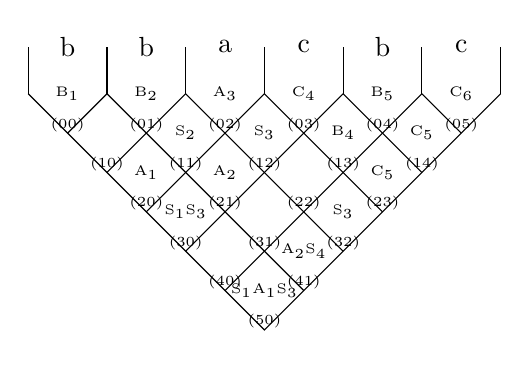
\begin{tikzpicture}[baseline]
			\newcommand{\myfontvars}[1]{
				\fontsize{4.9}{12}\selectfont{#1}
			}\newcommand{\myfontnumbering}[1]{
				\fontsize{2.5}{12}\selectfont{#1}
			}%Outer hull
			%Tip of the pyramid
			\coordinate (tip) at (3.0,-3.0);
			\foreach \i in {0,...,6} {
				\coordinate (\i) at (\i,0);
			}
			%Draw the left and right line of the pyramid pointing downwards
			\draw (0) -- (tip) -- (6);
			%Grid lines direction down-left to top-right
			\coordinate (dl1) at (0.5,-0.5);
			\coordinate (dl2) at (1.0,-1.0);
			\coordinate (dl3) at (1.5,-1.5);
			\coordinate (dl4) at (2.0,-2.0);
			\coordinate (dl5) at (2.5,-2.5);
			\draw (dl1) -- (1,0);
			\draw (dl2) -- (2,0);
			\draw (dl3) -- (3,0);
			\draw (dl4) -- (4,0);
			\draw (dl5) -- (5,0);
			%Grid lines direction down-right to top-left
			\coordinate (dr1) at (3.5,-2.5);
			\coordinate (dr2) at (4.0,-2.0);
			\coordinate (dr3) at (4.5,-1.5);
			\coordinate (dr4) at (5.0,-1.0);
			\coordinate (dr5) at (5.5,-0.5);
			\draw (dr1) -- (1,0);
			\draw (dr2) -- (2,0);
			\draw (dr3) -- (3,0);
			\draw (dr4) -- (4,0);
			\draw (dr5) -- (5,0);
			%Small lines at the top
			\coordinate (top0) at (0.0,0.0);
			\coordinate (top1) at (1.0,0.0);
			\coordinate (top2) at (2.0,0.0);
			\coordinate (top3) at (3.0,0.0);
			\coordinate (top4) at (4.0,0.0);
			\coordinate (top5) at (5.0,0.0);
			\coordinate (top6) at (6.0,0.0);
			\coordinate (topUpper0) at (0.0,0.6);
			\coordinate (topUpper1) at (1.0,0.6);
			\coordinate (topUpper2) at (2.0,0.6);
			\coordinate (topUpper3) at (3.0,0.6);
			\coordinate (topUpper4) at (4.0,0.6);
			\coordinate (topUpper5) at (5.0,0.6);
			\coordinate (topUpper6) at (6.0,0.6);
			\draw (top0) -- (topUpper0);
			\draw (top1) -- (topUpper1);
			\draw (top2) -- (topUpper2);
			\draw (top3) -- (topUpper3);
			\draw (top4) -- (topUpper4);
			\draw (top5) -- (topUpper5);
			\draw (top6) -- (topUpper6);
			%The string
			\coordinate (w0) at (0.5,0.6);
			\coordinate (w1) at (1.5,0.6);
			\coordinate (w2) at (2.5,0.6);
			\coordinate (w3) at (3.5,0.6);
			\coordinate (w4) at (4.5,0.6);
			\coordinate (w5) at (5.5,0.6);
			\node [] at (w0) {b};
			\node [] at (w1) {b};
			\node [] at (w2) {a};
			\node [] at (w3) {c};
			\node [] at (w4) {b};
			\node [] at (w5) {c};
			% Variables in the cells
			%cells00
			\coordinate (center00) at (0.5,0.0);
			\node [below=0.18cm] at (center00) {\myfontnumbering{$(00)$}};
			\node [] at (center00) {\myfontvars{B$_{1}$}};
			%cells01
			\coordinate (center01) at (1.5,0.0);
			\node [below=0.18cm] at (center01) {\myfontnumbering{$(01)$}};
			\node [] at (center01) {\myfontvars{B$_{2}$}};
			%cells02
			\coordinate (center02) at (2.5,0.0);
			\node [below=0.18cm] at (center02) {\myfontnumbering{$(02)$}};
			\node [] at (center02) {\myfontvars{A$_{3}$}};
			%cells03
			\coordinate (center03) at (3.5,0.0);
			\node [below=0.18cm] at (center03) {\myfontnumbering{$(03)$}};
			\node [] at (center03) {\myfontvars{C$_{4}$}};
			%cells04
			\coordinate (center04) at (4.5,0.0);
			\node [below=0.18cm] at (center04) {\myfontnumbering{$(04)$}};
			\node [] at (center04) {\myfontvars{B$_{5}$}};
			%cells05
			\coordinate (center05) at (5.5,0.0);
			\node [below=0.18cm] at (center05) {\myfontnumbering{$(05)$}};
			\node [] at (center05) {\myfontvars{C$_{6}$}};
			%cells10
			\coordinate (center10) at (1.0,-0.5);
			\node [below=0.18cm] at (center10) {\myfontnumbering{$(10)$}};
			%cells11
			\coordinate (center11) at (2.0,-0.5);
			\node [below=0.18cm] at (center11) {\myfontnumbering{$(11)$}};
			\node [] at (center11) {\myfontvars{S$_{2}$}};
			%cells12
			\coordinate (center12) at (3.0,-0.5);
			\node [below=0.18cm] at (center12) {\myfontnumbering{$(12)$}};
			\node [] at (center12) {\myfontvars{S$_{3}$}};
			%cells13
			\coordinate (center13) at (4.0,-0.5);
			\node [below=0.18cm] at (center13) {\myfontnumbering{$(13)$}};
			\node [] at (center13) {\myfontvars{B$_{4}$}};
			%cells14
			\coordinate (center14) at (5.0,-0.5);
			\node [below=0.18cm] at (center14) {\myfontnumbering{$(14)$}};
			\node [] at (center14) {\myfontvars{C$_{5}$}};
			%cells20
			\coordinate (center20) at (1.5,-1.0);
			\node [below=0.18cm] at (center20) {\myfontnumbering{$(20)$}};
			\node [] at (center20) {\myfontvars{A$_{1}$}};
			%cells21
			\coordinate (center21) at (2.5,-1.0);
			\node [below=0.18cm] at (center21) {\myfontnumbering{$(21)$}};
			\node [] at (center21) {\myfontvars{A$_{2}$}};
			%cells22
			\coordinate (center22) at (3.5,-1.0);
			\node [below=0.18cm] at (center22) {\myfontnumbering{$(22)$}};
			%cells23
			\coordinate (center23) at (4.5,-1.0);
			\node [below=0.18cm] at (center23) {\myfontnumbering{$(23)$}};
			\node [] at (center23) {\myfontvars{C$_{5}$}};
			%cells30
			\coordinate (center30) at (2.0,-1.5);
			\node [below=0.18cm] at (center30) {\myfontnumbering{$(30)$}};
			\node [] at (center30) {\myfontvars{S$_{1}$S$_{3}$}};
			%cells31
			\coordinate (center31) at (3.0,-1.5);
			\node [below=0.18cm] at (center31) {\myfontnumbering{$(31)$}};
			%cells32
			\coordinate (center32) at (4.0,-1.5);
			\node [below=0.18cm] at (center32) {\myfontnumbering{$(32)$}};
			\node [] at (center32) {\myfontvars{S$_{3}$}};
			%cells40
			\coordinate (center40) at (2.5,-2.0);
			\node [below=0.18cm] at (center40) {\myfontnumbering{$(40)$}};
			%cells41
			\coordinate (center41) at (3.5,-2.0);
			\node [below=0.18cm] at (center41) {\myfontnumbering{$(41)$}};
			\node [] at (center41) {\myfontvars{A$_{2}$S$_{4}$}};
			%cells50
			\coordinate (center50) at (3.0,-2.5);
			\node [below=0.18cm] at (center50) {\myfontnumbering{$(50)$}};
			\node [] at (center50) {\myfontvars{S$_{1}$A$_{1}$S$_{3}$}};
			\end{tikzpicture}
		}
	\end{minipage}
	\caption{Illustration of Algorithm \ref{SplitThenFill} SplitThenFill part 6. The recursion step in $Cell_{5,0}$ is  resolved by adding the rule $S\rightarrow AC$.}
	\label{IllustrationAlgorithmSplitThenFillPart6}
\end{figure}\\

\clearpage

\subsection{Split Top-Down and fill Top-Down}
After defining an algorithm that uses the combination of the Bottom-Up approach and the Top-Down approach (Algorithm \ref{SplitThenFill}) a step further is to find an algorithm that only makes use of the Top-Down approach to see if an even better algorithm can be found.\\
This algorithm again generates a predefined structure of the derivation tree Top-Downwards. Every time a node of the structure of the derivation tree has been decided on, a rule is immediately added to the grammar \textendash~therefore the name SplitAndFill, which is like "split for a node and then directly add a rule so that the node is then filled with at least one variable". \\
Note that the count of rules in the grammar is dependent on the count of nodes in the derivation tree and a terminal is distributed to only one variable. While resolving the last recursion step (Line \ref{splitAndFillRecLastStep}) of Algorithm \ref{SplitAndFillRecursion} SplitAndFillRec the start variable will be in the root of the pyramid that always leads to $w \in L(G)$.\\

\noindent
\frame{
	\begin{algorithm}[H] %or another one check
		\caption{SplitAndFill}
		\label{SplitAndFill}
		\SetAlgoLined
		\KwIn{Word $w \in \Sigma^{*}$}
		\KwOut{Set of productions $P$}
		$P = \emptyset$;~~\tcp{$P \subseteq V \times (V^{2} \cup \Sigma)$}
		$Sol = (P_{Sol},~v)$;~~\tcp{$P_{Sol} \subseteq P$} \label{splitAndFillcell}
		$Sol = SplitAndFillRec(P,\ w,\ i_{max},\ 0)$\;
		\Return $P_{Sol}$\;
				\footnotetext{
			\noindent Line \ref{splitAndFillcell}: $v$ can be any random element $v\in V$.
		}
	\end{algorithm}
}\\

\noindent
\frame{
	\begin{algorithm}[H] %or another one check
		\caption{SplitAndFillRec}
		\label{SplitAndFillRecursion}
		\SetAlgoLined
		\KwIn{$P_{in} \subseteq V \times (V^{2} \cup \Sigma),\ w \in \Sigma^{*},\ i,j \in \mathbb{N}$ }
		\KwOut{$(P,~v)$}
		$P = P_{in}$\;
		\If{$i=0$}{
			\If{terminal $w_j$ not distributed yet}{
				\Return $(P \cup \{(v,~ w_j)\},\ v_{lhse})$\; \label{termDistr1}	
			}
			\Return $(P,\ v_{lhse})$\;	\label{termDistr2}
		}
		$choose\ one\ m\ uniform\ randomly\ in\ [j+1,\ j+i]$\;
		$(P,\ v_l) = SplitAndFillRec(P,\ w,\ (m-j-1),\ j)$\label{left}\;
		$(P,\ v_r) = SplitAndFillRec(P,\ w,\ (j+i-m),\ m)$\label{right}\;	
		\If{$i=i_{max}$}{
			\Return $(P \cup \{(S,~v_l v_r)\},\ S)$\; \label{splitAndFillRecLastStep}
		}
		\Return $(P \cup \{(v,~v_l v_r)\},\ v)$\; \label{SplitAndFillReturn}
		\footnotetext{
			\noindent Line \ref{termDistr1} and Line \ref{termDistr2}: There is the rule $v_{lhse}\rightarrow w_j$, then $v_{lhse}$ is the variable on the left side of the one rule that has the terminal $w_j$ as its rhse.
			\noindent Line \ref{termDistr1} and Line \ref{SplitAndFillReturn}: $v$ is a random element $v\in V$.\\
		}
	\end{algorithm}
}
\\
According to this algorithm, only productions corresponding to the tree structure are added to the grammar. For illustration purposes, the pyramid is also shown to reflect the immediate changes of the added rules to the pyramid in the Figures \ref{IllustrationAlgorithmSplitAndFillPart1} to \ref{IllustrationAlgorithmSplitAndFillPart6}. Again the predefined derivation tree structure of Figure \ref{treeStruct} is used.
\noindent
\begin{figure} [h]
	\begin{minipage}{6in}
		\centering
		\begin{tabular}{l}
			Grammar:\\
			$A \rightarrow $\\
			$B \rightarrow b$\\ 
			$C \rightarrow $\\
			$S \rightarrow $\\ 
		\end{tabular} 
		\resizebox{0.65\linewidth}{!}{
		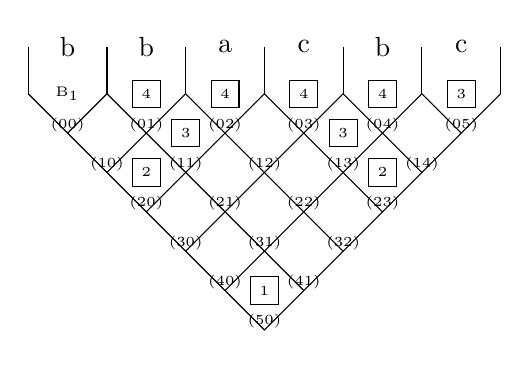
\begin{tikzpicture}[baseline]
		\newcommand{\myfontvars}[1]{
			\fontsize{4.9}{12}\selectfont{#1}
		}\newcommand{\myfontnumbering}[1]{
			\fontsize{2.5}{12}\selectfont{#1}
		}%Outer hull
		%Tip of the pyramid
		\coordinate (tip) at (3.0,-3.0);
		\foreach \i in {0,...,6} {
			\coordinate (\i) at (\i,0);
		}
		%Draw the left and right line of the pyramid pointing downwards
		\draw (0) -- (tip) -- (6);
		%Grid lines direction down-left to top-right
		\coordinate (dl1) at (0.5,-0.5);
		\coordinate (dl2) at (1.0,-1.0);
		\coordinate (dl3) at (1.5,-1.5);
		\coordinate (dl4) at (2.0,-2.0);
		\coordinate (dl5) at (2.5,-2.5);
		\draw (dl1) -- (1,0);
		\draw (dl2) -- (2,0);
		\draw (dl3) -- (3,0);
		\draw (dl4) -- (4,0);
		\draw (dl5) -- (5,0);
		%Grid lines direction down-right to top-left
		\coordinate (dr1) at (3.5,-2.5);
		\coordinate (dr2) at (4.0,-2.0);
		\coordinate (dr3) at (4.5,-1.5);
		\coordinate (dr4) at (5.0,-1.0);
		\coordinate (dr5) at (5.5,-0.5);
		\draw (dr1) -- (1,0);
		\draw (dr2) -- (2,0);
		\draw (dr3) -- (3,0);
		\draw (dr4) -- (4,0);
		\draw (dr5) -- (5,0);
		%Small lines at the top
		\coordinate (top0) at (0.0,0.0);
		\coordinate (top1) at (1.0,0.0);
		\coordinate (top2) at (2.0,0.0);
		\coordinate (top3) at (3.0,0.0);
		\coordinate (top4) at (4.0,0.0);
		\coordinate (top5) at (5.0,0.0);
		\coordinate (top6) at (6.0,0.0);
		\coordinate (topUpper0) at (0.0,0.6);
		\coordinate (topUpper1) at (1.0,0.6);
		\coordinate (topUpper2) at (2.0,0.6);
		\coordinate (topUpper3) at (3.0,0.6);
		\coordinate (topUpper4) at (4.0,0.6);
		\coordinate (topUpper5) at (5.0,0.6);
		\coordinate (topUpper6) at (6.0,0.6);
		\draw (top0) -- (topUpper0);
		\draw (top1) -- (topUpper1);
		\draw (top2) -- (topUpper2);
		\draw (top3) -- (topUpper3);
		\draw (top4) -- (topUpper4);
		\draw (top5) -- (topUpper5);
		\draw (top6) -- (topUpper6);
		%The string
		\coordinate (w0) at (0.5,0.6);
		\coordinate (w1) at (1.5,0.6);
		\coordinate (w2) at (2.5,0.6);
		\coordinate (w3) at (3.5,0.6);
		\coordinate (w4) at (4.5,0.6);
		\coordinate (w5) at (5.5,0.6);
		\node [] at (w0) {b};
		\node [] at (w1) {b};
		\node [] at (w2) {a};
		\node [] at (w3) {c};
		\node [] at (w4) {b};
		\node [] at (w5) {c};
		% Variables in the cells
		%cells00
		\coordinate (center00) at (0.5,0.0);
		\node [below=0.18cm] at (center00) {\myfontnumbering{$(00)$}};
		\node [] at (center00) {\myfontvars{B$_{1}$}};
		%cells01
		\coordinate (center01) at (1.5,0.0);
		\node [below=0.18cm] at (center01) {\myfontnumbering{$(01)$}};
		\node [] at (center01) [minimum height=0.25cm,minimum width=0.25cm,draw] {\tiny{4}};
		%cells02
		\coordinate (center02) at (2.5,0.0);
		\node [below=0.18cm] at (center02) {\myfontnumbering{$(02)$}};
		\node [] at (center02) [minimum height=0.25cm,minimum width=0.25cm,draw] {\tiny{4}};
		%cells03
		\coordinate (center03) at (3.5,0.0);
		\node [below=0.18cm] at (center03) {\myfontnumbering{$(03)$}};
		\node [] at (center03) [minimum height=0.25cm,minimum width=0.25cm,draw] {\tiny{4}};
		%cells04
		\coordinate (center04) at (4.5,0.0);
		\node [below=0.18cm] at (center04) {\myfontnumbering{$(04)$}};
		\node [] at (center04) [minimum height=0.25cm,minimum width=0.25cm,draw] {\tiny{4}};
		%cells05
		\coordinate (center05) at (5.5,0.0);
		\node [below=0.18cm] at (center05) {\myfontnumbering{$(05)$}};
		\node [] at (center05) [minimum height=0.25cm,minimum width=0.25cm,draw] {\tiny{3}};
		%cells10
		\coordinate (center10) at (1.0,-0.5);
		\node [below=0.18cm] at (center10) {\myfontnumbering{$(10)$}};
		%cells11
		\coordinate (center11) at (2.0,-0.5);
		\node [below=0.18cm] at (center11) {\myfontnumbering{$(11)$}};
		\node [] at (center11) [minimum height=0.25cm,minimum width=0.25cm,draw] {\tiny{3}};
		%cells12
		\coordinate (center12) at (3.0,-0.5);
		\node [below=0.18cm] at (center12) {\myfontnumbering{$(12)$}};
		%cells13
		\coordinate (center13) at (4.0,-0.5);
		\node [below=0.18cm] at (center13) {\myfontnumbering{$(13)$}};
		\node [] at (center13) [minimum height=0.25cm,minimum width=0.25cm,draw] {\tiny{3}};
		%cells14
		\coordinate (center14) at (5.0,-0.5);
		\node [below=0.18cm] at (center14) {\myfontnumbering{$(14)$}};
		%cells20
		\coordinate (center20) at (1.5,-1.0);
		\node [below=0.18cm] at (center20) {\myfontnumbering{$(20)$}};
		\node [] at (center20) [minimum height=0.25cm,minimum width=0.25cm,draw] {\tiny{2}};
		%cells21
		\coordinate (center21) at (2.5,-1.0);
		\node [below=0.18cm] at (center21) {\myfontnumbering{$(21)$}};
		%cells22
		\coordinate (center22) at (3.5,-1.0);
		\node [below=0.18cm] at (center22) {\myfontnumbering{$(22)$}};
		%cells23
		\coordinate (center23) at (4.5,-1.0);
		\node [below=0.18cm] at (center23) {\myfontnumbering{$(23)$}};
		\node [] at (center23) [minimum height=0.25cm,minimum width=0.25cm,draw] {\tiny{2}};
		%cells30
		\coordinate (center30) at (2.0,-1.5);
		\node [below=0.18cm] at (center30) {\myfontnumbering{$(30)$}};
		%cells31
		\coordinate (center31) at (3.0,-1.5);
		\node [below=0.18cm] at (center31) {\myfontnumbering{$(31)$}};
		%cells32
		\coordinate (center32) at (4.0,-1.5);
		\node [below=0.18cm] at (center32) {\myfontnumbering{$(32)$}};
		%cells40
		\coordinate (center40) at (2.5,-2.0);
		\node [below=0.18cm] at (center40) {\myfontnumbering{$(40)$}};
		%cells41
		\coordinate (center41) at (3.5,-2.0);
		\node [below=0.18cm] at (center41) {\myfontnumbering{$(41)$}};
		%cells50
		\coordinate (center50) at (3.0,-2.5);
		\node [below=0.18cm] at (center50) {\myfontnumbering{$(50)$}};
		\node [] at (center50) [minimum height=0.25cm,minimum width=0.25cm,draw] {\tiny{1}};
		\end{tikzpicture}
	}
	\end{minipage}
	\caption{Illustration of Algorithm \ref{SplitAndFill} part 1. To resolve the recursion step that fills $Cell_{0,0}$ the rule $B\rightarrow b$ is added.}
	\label{IllustrationAlgorithmSplitAndFillPart1}
\end{figure}

\noindent
\begin{figure} [h]
	\begin{minipage}{6in}
		\centering
		\begin{tabular}{l}
			Grammar:\\
			$A \rightarrow a$\\
			$B \rightarrow b$\\ 
			$C \rightarrow $\\
			$S \rightarrow BA$\\ 
		\end{tabular} 
		\resizebox{0.65\linewidth}{!}{
			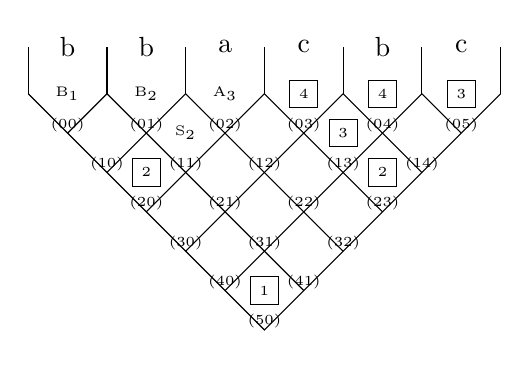
\begin{tikzpicture}[baseline]
			\newcommand{\myfontvars}[1]{
				\fontsize{4.9}{12}\selectfont{#1}
			}\newcommand{\myfontnumbering}[1]{
				\fontsize{2.5}{12}\selectfont{#1}
			}%Outer hull
			%Tip of the pyramid
			\coordinate (tip) at (3.0,-3.0);
			\foreach \i in {0,...,6} {
				\coordinate (\i) at (\i,0);
			}
			%Draw the left and right line of the pyramid pointing downwards
			\draw (0) -- (tip) -- (6);
			%Grid lines direction down-left to top-right
			\coordinate (dl1) at (0.5,-0.5);
			\coordinate (dl2) at (1.0,-1.0);
			\coordinate (dl3) at (1.5,-1.5);
			\coordinate (dl4) at (2.0,-2.0);
			\coordinate (dl5) at (2.5,-2.5);
			\draw (dl1) -- (1,0);
			\draw (dl2) -- (2,0);
			\draw (dl3) -- (3,0);
			\draw (dl4) -- (4,0);
			\draw (dl5) -- (5,0);
			%Grid lines direction down-right to top-left
			\coordinate (dr1) at (3.5,-2.5);
			\coordinate (dr2) at (4.0,-2.0);
			\coordinate (dr3) at (4.5,-1.5);
			\coordinate (dr4) at (5.0,-1.0);
			\coordinate (dr5) at (5.5,-0.5);
			\draw (dr1) -- (1,0);
			\draw (dr2) -- (2,0);
			\draw (dr3) -- (3,0);
			\draw (dr4) -- (4,0);
			\draw (dr5) -- (5,0);
			%Small lines at the top
			\coordinate (top0) at (0.0,0.0);
			\coordinate (top1) at (1.0,0.0);
			\coordinate (top2) at (2.0,0.0);
			\coordinate (top3) at (3.0,0.0);
			\coordinate (top4) at (4.0,0.0);
			\coordinate (top5) at (5.0,0.0);
			\coordinate (top6) at (6.0,0.0);
			\coordinate (topUpper0) at (0.0,0.6);
			\coordinate (topUpper1) at (1.0,0.6);
			\coordinate (topUpper2) at (2.0,0.6);
			\coordinate (topUpper3) at (3.0,0.6);
			\coordinate (topUpper4) at (4.0,0.6);
			\coordinate (topUpper5) at (5.0,0.6);
			\coordinate (topUpper6) at (6.0,0.6);
			\draw (top0) -- (topUpper0);
			\draw (top1) -- (topUpper1);
			\draw (top2) -- (topUpper2);
			\draw (top3) -- (topUpper3);
			\draw (top4) -- (topUpper4);
			\draw (top5) -- (topUpper5);
			\draw (top6) -- (topUpper6);
			%The string
			\coordinate (w0) at (0.5,0.6);
			\coordinate (w1) at (1.5,0.6);
			\coordinate (w2) at (2.5,0.6);
			\coordinate (w3) at (3.5,0.6);
			\coordinate (w4) at (4.5,0.6);
			\coordinate (w5) at (5.5,0.6);
			\node [] at (w0) {b};
			\node [] at (w1) {b};
			\node [] at (w2) {a};
			\node [] at (w3) {c};
			\node [] at (w4) {b};
			\node [] at (w5) {c};
			% Variables in the cells
			%cells00
			\coordinate (center00) at (0.5,0.0);
			\node [below=0.18cm] at (center00) {\myfontnumbering{$(00)$}};
			\node [] at (center00) {\myfontvars{B$_{1}$}};
			%cells01
			\coordinate (center01) at (1.5,0.0);
			\node [below=0.18cm] at (center01) {\myfontnumbering{$(01)$}};
			\node [] at (center01) {\myfontvars{B$_{2}$}};
			%cells02
			\coordinate (center02) at (2.5,0.0);
			\node [below=0.18cm] at (center02) {\myfontnumbering{$(02)$}};
			\node [] at (center02) {\myfontvars{A$_{3}$}};
			%cells03
			\coordinate (center03) at (3.5,0.0);
			\node [below=0.18cm] at (center03) {\myfontnumbering{$(03)$}};
			\node [] at (center03) [minimum height=0.25cm,minimum width=0.25cm,draw] {\tiny{4}};
			%cells04
			\coordinate (center04) at (4.5,0.0);
			\node [below=0.18cm] at (center04) {\myfontnumbering{$(04)$}};
			\node [] at (center04) [minimum height=0.25cm,minimum width=0.25cm,draw] {\tiny{4}};
			%cells05
			\coordinate (center05) at (5.5,0.0);
			\node [below=0.18cm] at (center05) {\myfontnumbering{$(05)$}};
			\node [] at (center05) [minimum height=0.25cm,minimum width=0.25cm,draw] {\tiny{3}};
			%cells10
			\coordinate (center10) at (1.0,-0.5);
			\node [below=0.18cm] at (center10) {\myfontnumbering{$(10)$}};
			%cells11
			\coordinate (center11) at (2.0,-0.5);
			\node [below=0.18cm] at (center11) {\myfontnumbering{$(11)$}};
			\node [] at (center11) {\myfontvars{S$_{2}$}};
			%cells12
			\coordinate (center12) at (3.0,-0.5);
			\node [below=0.18cm] at (center12) {\myfontnumbering{$(12)$}};
			%cells13
			\coordinate (center13) at (4.0,-0.5);
			\node [below=0.18cm] at (center13) {\myfontnumbering{$(13)$}};
			\node [] at (center13) [minimum height=0.25cm,minimum width=0.25cm,draw] {\tiny{3}};
			%cells14
			\coordinate (center14) at (5.0,-0.5);
			\node [below=0.18cm] at (center14) {\myfontnumbering{$(14)$}};
			%cells20
			\coordinate (center20) at (1.5,-1.0);
			\node [below=0.18cm] at (center20) {\myfontnumbering{$(20)$}};
			\node [] at (center20) [minimum height=0.25cm,minimum width=0.25cm,draw] {\tiny{2}};
			%cells21
			\coordinate (center21) at (2.5,-1.0);
			\node [below=0.18cm] at (center21) {\myfontnumbering{$(21)$}};
			%cells22
			\coordinate (center22) at (3.5,-1.0);
			\node [below=0.18cm] at (center22) {\myfontnumbering{$(22)$}};
			%cells23
			\coordinate (center23) at (4.5,-1.0);
			\node [below=0.18cm] at (center23) {\myfontnumbering{$(23)$}};
			\node [] at (center23) [minimum height=0.25cm,minimum width=0.25cm,draw] {\tiny{2}};
			%cells30
			\coordinate (center30) at (2.0,-1.5);
			\node [below=0.18cm] at (center30) {\myfontnumbering{$(30)$}};
			%cells31
			\coordinate (center31) at (3.0,-1.5);
			\node [below=0.18cm] at (center31) {\myfontnumbering{$(31)$}};
			%cells32
			\coordinate (center32) at (4.0,-1.5);
			\node [below=0.18cm] at (center32) {\myfontnumbering{$(32)$}};
			%cells40
			\coordinate (center40) at (2.5,-2.0);
			\node [below=0.18cm] at (center40) {\myfontnumbering{$(40)$}};
			%cells41
			\coordinate (center41) at (3.5,-2.0);
			\node [below=0.18cm] at (center41) {\myfontnumbering{$(41)$}};
			%cells50
			\coordinate (center50) at (3.0,-2.5);
			\node [below=0.18cm] at (center50) {\myfontnumbering{$(50)$}};
			\node [] at (center50) [minimum height=0.25cm,minimum width=0.25cm,draw] {\tiny{1}};
			\end{tikzpicture}
		}
	\end{minipage}
	\caption{Illustration of Algorithm \ref{SplitAndFill} part 2. Resolving the recursion step that fills $Cell_{0,1}$ no rule is added because a rule $lhse\rightarrow b$ already exists. To fill $Cell_{0,2}$ the rule $A\rightarrow a$ is added. Regarding $Cell_{1,1}$ the rule $S \rightarrow BA$ is added.}
	\label{IllustrationAlgorithmSplitAndFillPart2}
\end{figure}
\noindent
\begin{figure} [h]
	\begin{minipage}{6in}
		\centering
		\begin{tabular}{l}
			Grammar:\\
			$A \rightarrow a$\\
			$B \rightarrow b$\\ 
			$C \rightarrow BS$\\
			$S \rightarrow BA$\\ 
		\end{tabular} 
		\resizebox{0.65\linewidth}{!}{
			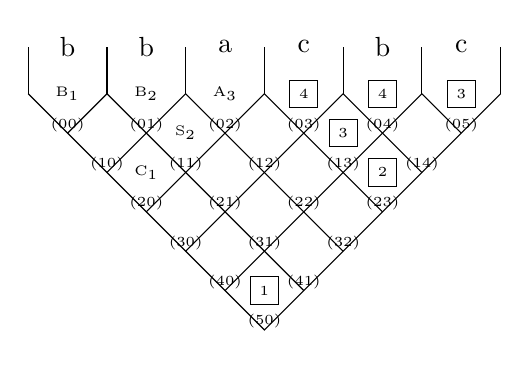
\begin{tikzpicture}[baseline]
			\newcommand{\myfontvars}[1]{
				\fontsize{4.9}{12}\selectfont{#1}
			}\newcommand{\myfontnumbering}[1]{
				\fontsize{2.5}{12}\selectfont{#1}
			}%Outer hull
			%Tip of the pyramid
			\coordinate (tip) at (3.0,-3.0);
			\foreach \i in {0,...,6} {
				\coordinate (\i) at (\i,0);
			}
			%Draw the left and right line of the pyramid pointing downwards
			\draw (0) -- (tip) -- (6);
			%Grid lines direction down-left to top-right
			\coordinate (dl1) at (0.5,-0.5);
			\coordinate (dl2) at (1.0,-1.0);
			\coordinate (dl3) at (1.5,-1.5);
			\coordinate (dl4) at (2.0,-2.0);
			\coordinate (dl5) at (2.5,-2.5);
			\draw (dl1) -- (1,0);
			\draw (dl2) -- (2,0);
			\draw (dl3) -- (3,0);
			\draw (dl4) -- (4,0);
			\draw (dl5) -- (5,0);
			%Grid lines direction down-right to top-left
			\coordinate (dr1) at (3.5,-2.5);
			\coordinate (dr2) at (4.0,-2.0);
			\coordinate (dr3) at (4.5,-1.5);
			\coordinate (dr4) at (5.0,-1.0);
			\coordinate (dr5) at (5.5,-0.5);
			\draw (dr1) -- (1,0);
			\draw (dr2) -- (2,0);
			\draw (dr3) -- (3,0);
			\draw (dr4) -- (4,0);
			\draw (dr5) -- (5,0);
			%Small lines at the top
			\coordinate (top0) at (0.0,0.0);
			\coordinate (top1) at (1.0,0.0);
			\coordinate (top2) at (2.0,0.0);
			\coordinate (top3) at (3.0,0.0);
			\coordinate (top4) at (4.0,0.0);
			\coordinate (top5) at (5.0,0.0);
			\coordinate (top6) at (6.0,0.0);
			\coordinate (topUpper0) at (0.0,0.6);
			\coordinate (topUpper1) at (1.0,0.6);
			\coordinate (topUpper2) at (2.0,0.6);
			\coordinate (topUpper3) at (3.0,0.6);
			\coordinate (topUpper4) at (4.0,0.6);
			\coordinate (topUpper5) at (5.0,0.6);
			\coordinate (topUpper6) at (6.0,0.6);
			\draw (top0) -- (topUpper0);
			\draw (top1) -- (topUpper1);
			\draw (top2) -- (topUpper2);
			\draw (top3) -- (topUpper3);
			\draw (top4) -- (topUpper4);
			\draw (top5) -- (topUpper5);
			\draw (top6) -- (topUpper6);
			%The string
			\coordinate (w0) at (0.5,0.6);
			\coordinate (w1) at (1.5,0.6);
			\coordinate (w2) at (2.5,0.6);
			\coordinate (w3) at (3.5,0.6);
			\coordinate (w4) at (4.5,0.6);
			\coordinate (w5) at (5.5,0.6);
			\node [] at (w0) {b};
			\node [] at (w1) {b};
			\node [] at (w2) {a};
			\node [] at (w3) {c};
			\node [] at (w4) {b};
			\node [] at (w5) {c};
			% Variables in the cells
			%cells00
			\coordinate (center00) at (0.5,0.0);
			\node [below=0.18cm] at (center00) {\myfontnumbering{$(00)$}};
			\node [] at (center00) {\myfontvars{B$_{1}$}};
			%cells01
			\coordinate (center01) at (1.5,0.0);
			\node [below=0.18cm] at (center01) {\myfontnumbering{$(01)$}};
			\node [] at (center01) {\myfontvars{B$_{2}$}};
			%cells02
			\coordinate (center02) at (2.5,0.0);
			\node [below=0.18cm] at (center02) {\myfontnumbering{$(02)$}};
			\node [] at (center02) {\myfontvars{A$_{3}$}};
			%cells03
			\coordinate (center03) at (3.5,0.0);
			\node [below=0.18cm] at (center03) {\myfontnumbering{$(03)$}};
			\node [] at (center03) [minimum height=0.25cm,minimum width=0.25cm,draw] {\tiny{4}};
			%cells04
			\coordinate (center04) at (4.5,0.0);
			\node [below=0.18cm] at (center04) {\myfontnumbering{$(04)$}};
			\node [] at (center04) [minimum height=0.25cm,minimum width=0.25cm,draw] {\tiny{4}};
			%cells05
			\coordinate (center05) at (5.5,0.0);
			\node [below=0.18cm] at (center05) {\myfontnumbering{$(05)$}};
			\node [] at (center05) [minimum height=0.25cm,minimum width=0.25cm,draw] {\tiny{3}};
			%cells10
			\coordinate (center10) at (1.0,-0.5);
			\node [below=0.18cm] at (center10) {\myfontnumbering{$(10)$}};
			%cells11
			\coordinate (center11) at (2.0,-0.5);
			\node [below=0.18cm] at (center11) {\myfontnumbering{$(11)$}};
			\node [] at (center11) {\myfontvars{S$_{2}$}};
			%cells12
			\coordinate (center12) at (3.0,-0.5);
			\node [below=0.18cm] at (center12) {\myfontnumbering{$(12)$}};
			%cells13
			\coordinate (center13) at (4.0,-0.5);
			\node [below=0.18cm] at (center13) {\myfontnumbering{$(13)$}};
			\node [] at (center13) [minimum height=0.25cm,minimum width=0.25cm,draw] {\tiny{3}};
			%cells14
			\coordinate (center14) at (5.0,-0.5);
			\node [below=0.18cm] at (center14) {\myfontnumbering{$(14)$}};
			%cells20
			\coordinate (center20) at (1.5,-1.0);
			\node [below=0.18cm] at (center20) {\myfontnumbering{$(20)$}};
			\node [] at (center20) {\myfontvars{C$_{1}$}};
			%cells21
			\coordinate (center21) at (2.5,-1.0);
			\node [below=0.18cm] at (center21) {\myfontnumbering{$(21)$}};
			%cells22
			\coordinate (center22) at (3.5,-1.0);
			\node [below=0.18cm] at (center22) {\myfontnumbering{$(22)$}};
			%cells23
			\coordinate (center23) at (4.5,-1.0);
			\node [below=0.18cm] at (center23) {\myfontnumbering{$(23)$}};
			\node [] at (center23) [minimum height=0.25cm,minimum width=0.25cm,draw] {\tiny{2}};
			%cells30
			\coordinate (center30) at (2.0,-1.5);
			\node [below=0.18cm] at (center30) {\myfontnumbering{$(30)$}};
			%cells31
			\coordinate (center31) at (3.0,-1.5);
			\node [below=0.18cm] at (center31) {\myfontnumbering{$(31)$}};
			%cells32
			\coordinate (center32) at (4.0,-1.5);
			\node [below=0.18cm] at (center32) {\myfontnumbering{$(32)$}};
			%cells40
			\coordinate (center40) at (2.5,-2.0);
			\node [below=0.18cm] at (center40) {\myfontnumbering{$(40)$}};
			%cells41
			\coordinate (center41) at (3.5,-2.0);
			\node [below=0.18cm] at (center41) {\myfontnumbering{$(41)$}};
			%cells50
			\coordinate (center50) at (3.0,-2.5);
			\node [below=0.18cm] at (center50) {\myfontnumbering{$(50)$}};
			\node [] at (center50) [minimum height=0.25cm,minimum width=0.25cm,draw] {\tiny{1}};
			\end{tikzpicture}
		}
	\end{minipage}
	\caption{Illustration of Algorithm \ref{SplitAndFill} part 3. Filling the $Cell_{2,0}$ the rule $C \rightarrow BS$ is added.}
	\label{IllustrationAlgorithmSplitAndFillPart3}
\end{figure}
\clearpage
\noindent
\begin{figure} [h]
	\begin{minipage}{6in}
		\centering
		\begin{tabular}{l}
			Grammar:\\
			$A \rightarrow BC~|~a$\\
			$B \rightarrow CB~|~b$\\ 
			$C \rightarrow BS~|~c$\\
			$S \rightarrow BA$\\ 
		\end{tabular} 
		\resizebox{0.65\linewidth}{!}{
			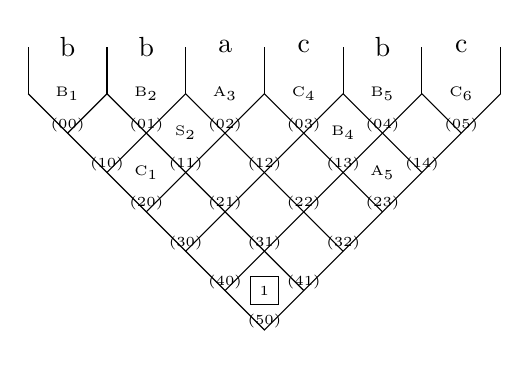
\begin{tikzpicture}[baseline]
			\newcommand{\myfontvars}[1]{
				\fontsize{4.9}{12}\selectfont{#1}
			}\newcommand{\myfontnumbering}[1]{
				\fontsize{2.5}{12}\selectfont{#1}
			}%Outer hull
			%Tip of the pyramid
			\coordinate (tip) at (3.0,-3.0);
			\foreach \i in {0,...,6} {
				\coordinate (\i) at (\i,0);
			}
			%Draw the left and right line of the pyramid pointing downwards
			\draw (0) -- (tip) -- (6);
			%Grid lines direction down-left to top-right
			\coordinate (dl1) at (0.5,-0.5);
			\coordinate (dl2) at (1.0,-1.0);
			\coordinate (dl3) at (1.5,-1.5);
			\coordinate (dl4) at (2.0,-2.0);
			\coordinate (dl5) at (2.5,-2.5);
			\draw (dl1) -- (1,0);
			\draw (dl2) -- (2,0);
			\draw (dl3) -- (3,0);
			\draw (dl4) -- (4,0);
			\draw (dl5) -- (5,0);
			%Grid lines direction down-right to top-left
			\coordinate (dr1) at (3.5,-2.5);
			\coordinate (dr2) at (4.0,-2.0);
			\coordinate (dr3) at (4.5,-1.5);
			\coordinate (dr4) at (5.0,-1.0);
			\coordinate (dr5) at (5.5,-0.5);
			\draw (dr1) -- (1,0);
			\draw (dr2) -- (2,0);
			\draw (dr3) -- (3,0);
			\draw (dr4) -- (4,0);
			\draw (dr5) -- (5,0);
			%Small lines at the top
			\coordinate (top0) at (0.0,0.0);
			\coordinate (top1) at (1.0,0.0);
			\coordinate (top2) at (2.0,0.0);
			\coordinate (top3) at (3.0,0.0);
			\coordinate (top4) at (4.0,0.0);
			\coordinate (top5) at (5.0,0.0);
			\coordinate (top6) at (6.0,0.0);
			\coordinate (topUpper0) at (0.0,0.6);
			\coordinate (topUpper1) at (1.0,0.6);
			\coordinate (topUpper2) at (2.0,0.6);
			\coordinate (topUpper3) at (3.0,0.6);
			\coordinate (topUpper4) at (4.0,0.6);
			\coordinate (topUpper5) at (5.0,0.6);
			\coordinate (topUpper6) at (6.0,0.6);
			\draw (top0) -- (topUpper0);
			\draw (top1) -- (topUpper1);
			\draw (top2) -- (topUpper2);
			\draw (top3) -- (topUpper3);
			\draw (top4) -- (topUpper4);
			\draw (top5) -- (topUpper5);
			\draw (top6) -- (topUpper6);
			%The string
			\coordinate (w0) at (0.5,0.6);
			\coordinate (w1) at (1.5,0.6);
			\coordinate (w2) at (2.5,0.6);
			\coordinate (w3) at (3.5,0.6);
			\coordinate (w4) at (4.5,0.6);
			\coordinate (w5) at (5.5,0.6);
			\node [] at (w0) {b};
			\node [] at (w1) {b};
			\node [] at (w2) {a};
			\node [] at (w3) {c};
			\node [] at (w4) {b};
			\node [] at (w5) {c};
			% Variables in the cells
			%cells00
			\coordinate (center00) at (0.5,0.0);
			\node [below=0.18cm] at (center00) {\myfontnumbering{$(00)$}};
			\node [] at (center00) {\myfontvars{B$_{1}$}};
			%cells01
			\coordinate (center01) at (1.5,0.0);
			\node [below=0.18cm] at (center01) {\myfontnumbering{$(01)$}};
			\node [] at (center01) {\myfontvars{B$_{2}$}};
			%cells02
			\coordinate (center02) at (2.5,0.0);
			\node [below=0.18cm] at (center02) {\myfontnumbering{$(02)$}};
			\node [] at (center02) {\myfontvars{A$_{3}$}};
			%cells03
			\coordinate (center03) at (3.5,0.0);
			\node [below=0.18cm] at (center03) {\myfontnumbering{$(03)$}};
			\node [] at (center03) {\myfontvars{C$_{4}$}};
			%cells04
			\coordinate (center04) at (4.5,0.0);
			\node [below=0.18cm] at (center04) {\myfontnumbering{$(04)$}};
			\node [] at (center04) {\myfontvars{B$_{5}$}};
			%cells05
			\coordinate (center05) at (5.5,0.0);
			\node [below=0.18cm] at (center05) {\myfontnumbering{$(05)$}};
			\node [] at (center05) {\myfontvars{C$_{6}$}};
			%cells10
			\coordinate (center10) at (1.0,-0.5);
			\node [below=0.18cm] at (center10) {\myfontnumbering{$(10)$}};
			%cells11
			\coordinate (center11) at (2.0,-0.5);
			\node [below=0.18cm] at (center11) {\myfontnumbering{$(11)$}};
			\node [] at (center11) {\myfontvars{S$_{2}$}};
			%cells12
			\coordinate (center12) at (3.0,-0.5);
			\node [below=0.18cm] at (center12) {\myfontnumbering{$(12)$}};
			%cells13
			\coordinate (center13) at (4.0,-0.5);
			\node [below=0.18cm] at (center13) {\myfontnumbering{$(13)$}};
			\node [] at (center13) {\myfontvars{B$_{4}$}};
			%cells14
			\coordinate (center14) at (5.0,-0.5);
			\node [below=0.18cm] at (center14) {\myfontnumbering{$(14)$}};
			%cells20
			\coordinate (center20) at (1.5,-1.0);
			\node [below=0.18cm] at (center20) {\myfontnumbering{$(20)$}};
			\node [] at (center20) {\myfontvars{C$_{1}$}};
			%cells21
			\coordinate (center21) at (2.5,-1.0);
			\node [below=0.18cm] at (center21) {\myfontnumbering{$(21)$}};
			%cells22
			\coordinate (center22) at (3.5,-1.0);
			\node [below=0.18cm] at (center22) {\myfontnumbering{$(22)$}};
			%cells23
			\coordinate (center23) at (4.5,-1.0);
			\node [below=0.18cm] at (center23) {\myfontnumbering{$(23)$}};
			\node [] at (center23) {\myfontvars{A$_{5}$}};
			%cells30
			\coordinate (center30) at (2.0,-1.5);
			\node [below=0.18cm] at (center30) {\myfontnumbering{$(30)$}};
			%cells31
			\coordinate (center31) at (3.0,-1.5);
			\node [below=0.18cm] at (center31) {\myfontnumbering{$(31)$}};
			%cells32
			\coordinate (center32) at (4.0,-1.5);
			\node [below=0.18cm] at (center32) {\myfontnumbering{$(32)$}};
			%cells40
			\coordinate (center40) at (2.5,-2.0);
			\node [below=0.18cm] at (center40) {\myfontnumbering{$(40)$}};
			%cells41
			\coordinate (center41) at (3.5,-2.0);
			\node [below=0.18cm] at (center41) {\myfontnumbering{$(41)$}};
			%cells50
			\coordinate (center50) at (3.0,-2.5);
			\node [below=0.18cm] at (center50) {\myfontnumbering{$(50)$}};
			\node [] at (center50) [minimum height=0.25cm,minimum width=0.25cm,draw] {\tiny{1}};
			\end{tikzpicture}
		}
	\end{minipage}
	\caption{Illustration of Algorithm \ref{SplitAndFill} part 4. Analogously the other cells are filled. $Cell_{0,3}$ is responsible for the rule $C \rightarrow c$, $Cell_{0,4}$ doesn't cause a rule because again there already is the rule $B \rightarrow b$, $Cell_{1,3}$ contributes for the rule $B \rightarrow CB$, $Cell_{0,5}$ does not add a rule because of $C\rightarrow c$ and to fill $Cell_{2,3}$ the rule $A \rightarrow BC$ is added.}
	\label{IllustrationAlgorithmSplitAndFillPart4}
\end{figure}

\noindent
\begin{figure} [h]
	\begin{minipage}{6in}
		\centering
		\begin{tabular}{l}
			Grammar:\\
			$A \rightarrow BC~|~a$\\
			$B \rightarrow CB~|~b$\\ 
			$C \rightarrow BS~|~c$\\
			$S \rightarrow BA~|~CA$\\ 
		\end{tabular} 
		\resizebox{0.65\linewidth}{!}{
			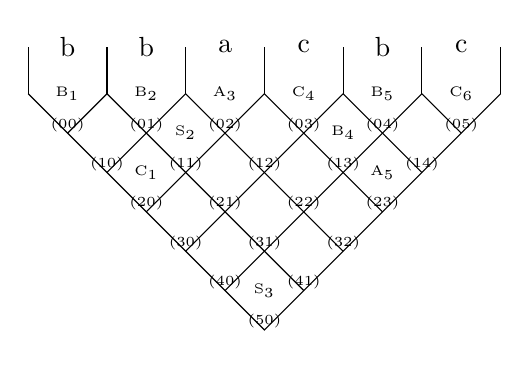
\begin{tikzpicture}[baseline]
			\newcommand{\myfontvars}[1]{
				\fontsize{4.9}{12}\selectfont{#1}
			}\newcommand{\myfontnumbering}[1]{
				\fontsize{2.5}{12}\selectfont{#1}
			}%Outer hull
			%Tip of the pyramid
			\coordinate (tip) at (3.0,-3.0);
			\foreach \i in {0,...,6} {
				\coordinate (\i) at (\i,0);
			}
			%Draw the left and right line of the pyramid pointing downwards
			\draw (0) -- (tip) -- (6);
			%Grid lines direction down-left to top-right
			\coordinate (dl1) at (0.5,-0.5);
			\coordinate (dl2) at (1.0,-1.0);
			\coordinate (dl3) at (1.5,-1.5);
			\coordinate (dl4) at (2.0,-2.0);
			\coordinate (dl5) at (2.5,-2.5);
			\draw (dl1) -- (1,0);
			\draw (dl2) -- (2,0);
			\draw (dl3) -- (3,0);
			\draw (dl4) -- (4,0);
			\draw (dl5) -- (5,0);
			%Grid lines direction down-right to top-left
			\coordinate (dr1) at (3.5,-2.5);
			\coordinate (dr2) at (4.0,-2.0);
			\coordinate (dr3) at (4.5,-1.5);
			\coordinate (dr4) at (5.0,-1.0);
			\coordinate (dr5) at (5.5,-0.5);
			\draw (dr1) -- (1,0);
			\draw (dr2) -- (2,0);
			\draw (dr3) -- (3,0);
			\draw (dr4) -- (4,0);
			\draw (dr5) -- (5,0);
			%Small lines at the top
			\coordinate (top0) at (0.0,0.0);
			\coordinate (top1) at (1.0,0.0);
			\coordinate (top2) at (2.0,0.0);
			\coordinate (top3) at (3.0,0.0);
			\coordinate (top4) at (4.0,0.0);
			\coordinate (top5) at (5.0,0.0);
			\coordinate (top6) at (6.0,0.0);
			\coordinate (topUpper0) at (0.0,0.6);
			\coordinate (topUpper1) at (1.0,0.6);
			\coordinate (topUpper2) at (2.0,0.6);
			\coordinate (topUpper3) at (3.0,0.6);
			\coordinate (topUpper4) at (4.0,0.6);
			\coordinate (topUpper5) at (5.0,0.6);
			\coordinate (topUpper6) at (6.0,0.6);
			\draw (top0) -- (topUpper0);
			\draw (top1) -- (topUpper1);
			\draw (top2) -- (topUpper2);
			\draw (top3) -- (topUpper3);
			\draw (top4) -- (topUpper4);
			\draw (top5) -- (topUpper5);
			\draw (top6) -- (topUpper6);
			%The string
			\coordinate (w0) at (0.5,0.6);
			\coordinate (w1) at (1.5,0.6);
			\coordinate (w2) at (2.5,0.6);
			\coordinate (w3) at (3.5,0.6);
			\coordinate (w4) at (4.5,0.6);
			\coordinate (w5) at (5.5,0.6);
			\node [] at (w0) {b};
			\node [] at (w1) {b};
			\node [] at (w2) {a};
			\node [] at (w3) {c};
			\node [] at (w4) {b};
			\node [] at (w5) {c};
			% Variables in the cells
			%cells00
			\coordinate (center00) at (0.5,0.0);
			\node [below=0.18cm] at (center00) {\myfontnumbering{$(00)$}};
			\node [] at (center00) {\myfontvars{B$_{1}$}};
			%cells01
			\coordinate (center01) at (1.5,0.0);
			\node [below=0.18cm] at (center01) {\myfontnumbering{$(01)$}};
			\node [] at (center01) {\myfontvars{B$_{2}$}};
			%cells02
			\coordinate (center02) at (2.5,0.0);
			\node [below=0.18cm] at (center02) {\myfontnumbering{$(02)$}};
			\node [] at (center02) {\myfontvars{A$_{3}$}};
			%cells03
			\coordinate (center03) at (3.5,0.0);
			\node [below=0.18cm] at (center03) {\myfontnumbering{$(03)$}};
			\node [] at (center03) {\myfontvars{C$_{4}$}};
			%cells04
			\coordinate (center04) at (4.5,0.0);
			\node [below=0.18cm] at (center04) {\myfontnumbering{$(04)$}};
			\node [] at (center04) {\myfontvars{B$_{5}$}};
			%cells05
			\coordinate (center05) at (5.5,0.0);
			\node [below=0.18cm] at (center05) {\myfontnumbering{$(05)$}};
			\node [] at (center05) {\myfontvars{C$_{6}$}};
			%cells10
			\coordinate (center10) at (1.0,-0.5);
			\node [below=0.18cm] at (center10) {\myfontnumbering{$(10)$}};
			%cells11
			\coordinate (center11) at (2.0,-0.5);
			\node [below=0.18cm] at (center11) {\myfontnumbering{$(11)$}};
			\node [] at (center11) {\myfontvars{S$_{2}$}};
			%cells12
			\coordinate (center12) at (3.0,-0.5);
			\node [below=0.18cm] at (center12) {\myfontnumbering{$(12)$}};
			%cells13
			\coordinate (center13) at (4.0,-0.5);
			\node [below=0.18cm] at (center13) {\myfontnumbering{$(13)$}};
			\node [] at (center13) {\myfontvars{B$_{4}$}};
			%cells14
			\coordinate (center14) at (5.0,-0.5);
			\node [below=0.18cm] at (center14) {\myfontnumbering{$(14)$}};
			%cells20
			\coordinate (center20) at (1.5,-1.0);
			\node [below=0.18cm] at (center20) {\myfontnumbering{$(20)$}};
			\node [] at (center20) {\myfontvars{C$_{1}$}};
			%cells21
			\coordinate (center21) at (2.5,-1.0);
			\node [below=0.18cm] at (center21) {\myfontnumbering{$(21)$}};
			%cells22
			\coordinate (center22) at (3.5,-1.0);
			\node [below=0.18cm] at (center22) {\myfontnumbering{$(22)$}};
			%cells23
			\coordinate (center23) at (4.5,-1.0);
			\node [below=0.18cm] at (center23) {\myfontnumbering{$(23)$}};
			\node [] at (center23) {\myfontvars{A$_{5}$}};
			%cells30
			\coordinate (center30) at (2.0,-1.5);
			\node [below=0.18cm] at (center30) {\myfontnumbering{$(30)$}};
			%cells31
			\coordinate (center31) at (3.0,-1.5);
			\node [below=0.18cm] at (center31) {\myfontnumbering{$(31)$}};
			%cells32
			\coordinate (center32) at (4.0,-1.5);
			\node [below=0.18cm] at (center32) {\myfontnumbering{$(32)$}};
			%cells40
			\coordinate (center40) at (2.5,-2.0);
			\node [below=0.18cm] at (center40) {\myfontnumbering{$(40)$}};
			%cells41
			\coordinate (center41) at (3.5,-2.0);
			\node [below=0.18cm] at (center41) {\myfontnumbering{$(41)$}};
			%cells50
			\coordinate (center50) at (3.0,-2.5);
			\node [below=0.18cm] at (center50) {\myfontnumbering{$(50)$}};
			\node [] at (center50) {\myfontvars{S$_{3}$}};
			\end{tikzpicture}
		}
	\end{minipage}
	\caption{Illustration of Algorithm \ref{SplitAndFill} part 5. Finally, to fill the cell in the root a rule must be added that has the start variable as its $lhse$ that guarantees $w \in L(G)$. Here the rule $S\rightarrow CA$ is added.}
	\label{IllustrationAlgorithmSplitAndFillPart5}
\end{figure}

\clearpage

\noindent
\begin{figure} [h]
	\begin{minipage}{6in}
		\centering
		\begin{tabular}{l}
			Grammar:\\
			$A \rightarrow BC~|~a$\\
			$B \rightarrow CB~|~b$\\ 
			$C \rightarrow BS~|~c$\\
			$S \rightarrow BA~|~CA$\\ 
		\end{tabular} 
		\resizebox{0.65\linewidth}{!}{
			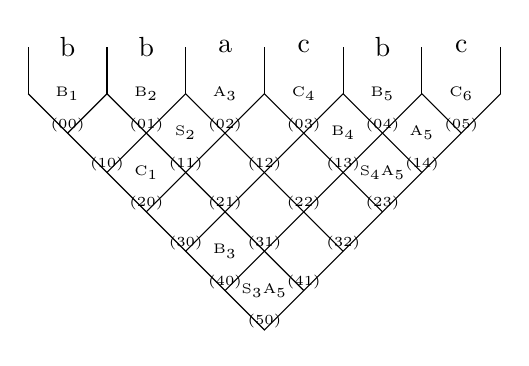
\begin{tikzpicture}[baseline]
			\newcommand{\myfontvars}[1]{
				\fontsize{4.9}{12}\selectfont{#1}
			}\newcommand{\myfontnumbering}[1]{
				\fontsize{2.5}{12}\selectfont{#1}
			}%Outer hull
			%Tip of the pyramid
			\coordinate (tip) at (3.0,-3.0);
			\foreach \i in {0,...,6} {
				\coordinate (\i) at (\i,0);
			}
			%Draw the left and right line of the pyramid pointing downwards
			\draw (0) -- (tip) -- (6);
			%Grid lines direction down-left to top-right
			\coordinate (dl1) at (0.5,-0.5);
			\coordinate (dl2) at (1.0,-1.0);
			\coordinate (dl3) at (1.5,-1.5);
			\coordinate (dl4) at (2.0,-2.0);
			\coordinate (dl5) at (2.5,-2.5);
			\draw (dl1) -- (1,0);
			\draw (dl2) -- (2,0);
			\draw (dl3) -- (3,0);
			\draw (dl4) -- (4,0);
			\draw (dl5) -- (5,0);
			%Grid lines direction down-right to top-left
			\coordinate (dr1) at (3.5,-2.5);
			\coordinate (dr2) at (4.0,-2.0);
			\coordinate (dr3) at (4.5,-1.5);
			\coordinate (dr4) at (5.0,-1.0);
			\coordinate (dr5) at (5.5,-0.5);
			\draw (dr1) -- (1,0);
			\draw (dr2) -- (2,0);
			\draw (dr3) -- (3,0);
			\draw (dr4) -- (4,0);
			\draw (dr5) -- (5,0);
			%Small lines at the top
			\coordinate (top0) at (0.0,0.0);
			\coordinate (top1) at (1.0,0.0);
			\coordinate (top2) at (2.0,0.0);
			\coordinate (top3) at (3.0,0.0);
			\coordinate (top4) at (4.0,0.0);
			\coordinate (top5) at (5.0,0.0);
			\coordinate (top6) at (6.0,0.0);
			\coordinate (topUpper0) at (0.0,0.6);
			\coordinate (topUpper1) at (1.0,0.6);
			\coordinate (topUpper2) at (2.0,0.6);
			\coordinate (topUpper3) at (3.0,0.6);
			\coordinate (topUpper4) at (4.0,0.6);
			\coordinate (topUpper5) at (5.0,0.6);
			\coordinate (topUpper6) at (6.0,0.6);
			\draw (top0) -- (topUpper0);
			\draw (top1) -- (topUpper1);
			\draw (top2) -- (topUpper2);
			\draw (top3) -- (topUpper3);
			\draw (top4) -- (topUpper4);
			\draw (top5) -- (topUpper5);
			\draw (top6) -- (topUpper6);
			%The string
			\coordinate (w0) at (0.5,0.6);
			\coordinate (w1) at (1.5,0.6);
			\coordinate (w2) at (2.5,0.6);
			\coordinate (w3) at (3.5,0.6);
			\coordinate (w4) at (4.5,0.6);
			\coordinate (w5) at (5.5,0.6);
			\node [] at (w0) {b};
			\node [] at (w1) {b};
			\node [] at (w2) {a};
			\node [] at (w3) {c};
			\node [] at (w4) {b};
			\node [] at (w5) {c};
			% Variables in the cells
			%cells00
			\coordinate (center00) at (0.5,0.0);
			\node [below=0.18cm] at (center00) {\myfontnumbering{$(00)$}};
			\node [] at (center00) {\myfontvars{B$_{1}$}};
			%cells01
			\coordinate (center01) at (1.5,0.0);
			\node [below=0.18cm] at (center01) {\myfontnumbering{$(01)$}};
			\node [] at (center01) {\myfontvars{B$_{2}$}};
			%cells02
			\coordinate (center02) at (2.5,0.0);
			\node [below=0.18cm] at (center02) {\myfontnumbering{$(02)$}};
			\node [] at (center02) {\myfontvars{A$_{3}$}};
			%cells03
			\coordinate (center03) at (3.5,0.0);
			\node [below=0.18cm] at (center03) {\myfontnumbering{$(03)$}};
			\node [] at (center03) {\myfontvars{C$_{4}$}};
			%cells04
			\coordinate (center04) at (4.5,0.0);
			\node [below=0.18cm] at (center04) {\myfontnumbering{$(04)$}};
			\node [] at (center04) {\myfontvars{B$_{5}$}};
			%cells05
			\coordinate (center05) at (5.5,0.0);
			\node [below=0.18cm] at (center05) {\myfontnumbering{$(05)$}};
			\node [] at (center05) {\myfontvars{C$_{6}$}};
			%cells10
			\coordinate (center10) at (1.0,-0.5);
			\node [below=0.18cm] at (center10) {\myfontnumbering{$(10)$}};
			%cells11
			\coordinate (center11) at (2.0,-0.5);
			\node [below=0.18cm] at (center11) {\myfontnumbering{$(11)$}};
			\node [] at (center11) {\myfontvars{S$_{2}$}};
			%cells12
			\coordinate (center12) at (3.0,-0.5);
			\node [below=0.18cm] at (center12) {\myfontnumbering{$(12)$}};
			%cells13
			\coordinate (center13) at (4.0,-0.5);
			\node [below=0.18cm] at (center13) {\myfontnumbering{$(13)$}};
			\node [] at (center13) {\myfontvars{B$_{4}$}};
			%cells14
			\coordinate (center14) at (5.0,-0.5);
			\node [below=0.18cm] at (center14) {\myfontnumbering{$(14)$}};
			\node [] at (center14) {\myfontvars{A$_{5}$}};
			%cells20
			\coordinate (center20) at (1.5,-1.0);
			\node [below=0.18cm] at (center20) {\myfontnumbering{$(20)$}};
			\node [] at (center20) {\myfontvars{C$_{1}$}};
			%cells21
			\coordinate (center21) at (2.5,-1.0);
			\node [below=0.18cm] at (center21) {\myfontnumbering{$(21)$}};
			%cells22
			\coordinate (center22) at (3.5,-1.0);
			\node [below=0.18cm] at (center22) {\myfontnumbering{$(22)$}};
			%cells23
			\coordinate (center23) at (4.5,-1.0);
			\node [below=0.18cm] at (center23) {\myfontnumbering{$(23)$}};
			\node [] at (center23) {\myfontvars{S$_{4}$A$_{5}$}};
			%cells30
			\coordinate (center30) at (2.0,-1.5);
			\node [below=0.18cm] at (center30) {\myfontnumbering{$(30)$}};
			%cells31
			\coordinate (center31) at (3.0,-1.5);
			\node [below=0.18cm] at (center31) {\myfontnumbering{$(31)$}};
			%cells32
			\coordinate (center32) at (4.0,-1.5);
			\node [below=0.18cm] at (center32) {\myfontnumbering{$(32)$}};
			%cells40
			\coordinate (center40) at (2.5,-2.0);
			\node [below=0.18cm] at (center40) {\myfontnumbering{$(40)$}};
			\node [] at (center40) {\myfontvars{B$_{3}$}};
			%cells41
			\coordinate (center41) at (3.5,-2.0);
			\node [below=0.18cm] at (center41) {\myfontnumbering{$(41)$}};
			%cells50
			\coordinate (center50) at (3.0,-2.5);
			\node [below=0.18cm] at (center50) {\myfontnumbering{$(50)$}};
			\node [] at (center50) {\myfontvars{S$_{3}$A$_{5}$}};
			\end{tikzpicture}
		}
	\end{minipage}
	\caption{Illustration of Algorithm \ref{SplitAndFill} part 6. With part 5 of the example the algorithm is finished. In comparison to Figure \ref{IllustrationAlgorithmSplitAndFillPart5} the complete parsing table looks like above.}
	\label{IllustrationAlgorithmSplitAndFillPart6}
\end{figure}

\clearpage
\pagebreak
\subsection{Evaluation of Algorithms} \label{AnalysisOfAlgorithms}
\subsubsection{Success Rates} \label{successRates}
\noindent Until now different algorithms have been described that could be used in the application to create suitable exam $exercises$. But it is of interest to find out which algorithm performs the best and which algorithm should actually be used in the application to generate the $exercise$s. Therefore a composite $Success~Rate$ is defined that measures the algorithms performance for the different requirements towards an exam $exercise$.  \\

\noindent Here $N \in  \mathbb{N}$ is the sample size of all generated grammars while examining the algorithms. Before defining the overall Success Rate ($SR$) three other Success Rates set the basis for it.\\

\noindent\textbf{Success Rate Producibility: }
A generated $exercise$ contributes to the SR-Producibility if the CYK algorithm's output (Algorithm \ref{CYK}) is true or in other words $w\in L(G)$.\\
SR-Producibility $ = p / N$, where $p$ is the count of $exercise$s that fulfil the requirement.\\

\noindent\textbf{Success Rate Cardinality-Rules: }
A generated $exercise$ contributes to the SR-Cardinality-Rules if the grammar has less than a certain count $x$ of rules, i.e. $|P|\leq x$ of the grammar $G=(V,\ \Sigma,\ S,\ P)$.\\
SR-Cardinality-Rules $ = cr / N$, where $cr$ is the count of $exercise$s.\\

\noindent\textbf{Success Rate Pyramid: }
A generated $exercise$ contributes to the SR-Pyramid if the following conditions are met:
\begin{enumerate} [noitemsep]
	\item At least one cell enforces to do a correct cell combination \textendash~see the description of Algorithm \ref{checkForceCombinationPerCell} CheckforceCombinationPerCell for more information.
	\item There are less than 100 variables in the entire pyramid.
	\item There are less than 3 variables in each cell of the pyramid.
\end{enumerate}
SR-Pyramid $= p / N$, where $p$ is the count of $exercise$s that fulfil the three requirements above. \\

\noindent For the sake of these checks (1., 2. and 3.) the definition of a $cell$ in the $pyramid$ is simplified as following:\\ 
$Cell_{i,j} \subseteq \{(V,k)~|~k \in \mathbb{N} \} \longrightarrow Cell_{i,j} \subseteq V$\\
For further illustration see Figure \ref{simplificationExample} on the next page. 
\clearpage
\noindent 
\begin{figure}[h]
	\begin{minipage}{6in}
		\centering
		\raisebox{-0.5\height}{
			\resizebox{0.45\linewidth}{!}{
				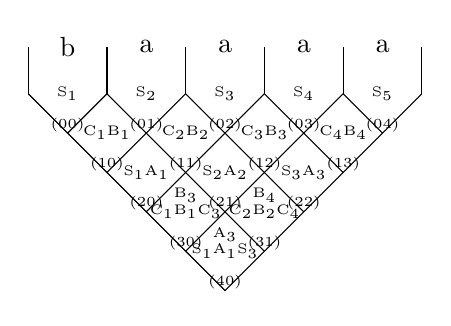
\begin{tikzpicture}[baseline]
				\newcommand{\myfontvars}[1]{
					\fontsize{4.9}{12}\selectfont{#1}
				}\newcommand{\myfontnumbering}[1]{
					\fontsize{2.5}{12}\selectfont{#1}
				}%Outer hull
				%Tip of the pyramid
				\coordinate (tip) at (2.5,-2.5);
				\foreach \i in {0,...,5} {
					\coordinate (\i) at (\i,0);
				}
				%Draw the left and right line of the pyramid pointing downwards
				\draw (0) -- (tip) -- (5);
				%Grid lines direction down-left to top-right
				\coordinate (dl1) at (0.5,-0.5);
				\coordinate (dl2) at (1.0,-1.0);
				\coordinate (dl3) at (1.5,-1.5);
				\coordinate (dl4) at (2.0,-2.0);
				\draw (dl1) -- (1,0);
				\draw (dl2) -- (2,0);
				\draw (dl3) -- (3,0);
				\draw (dl4) -- (4,0);
				%Grid lines direction down-right to top-left
				\coordinate (dr1) at (3.0,-2.0);
				\coordinate (dr2) at (3.5,-1.5);
				\coordinate (dr3) at (4.0,-1.0);
				\coordinate (dr4) at (4.5,-0.5);
				\draw (dr1) -- (1,0);
				\draw (dr2) -- (2,0);
				\draw (dr3) -- (3,0);
				\draw (dr4) -- (4,0);
				%Small lines at the top
				\coordinate (top0) at (0.0,0.0);
				\coordinate (top1) at (1.0,0.0);
				\coordinate (top2) at (2.0,0.0);
				\coordinate (top3) at (3.0,0.0);
				\coordinate (top4) at (4.0,0.0);
				\coordinate (top5) at (5.0,0.0);
				\coordinate (topUpper0) at (0.0,0.6);
				\coordinate (topUpper1) at (1.0,0.6);
				\coordinate (topUpper2) at (2.0,0.6);
				\coordinate (topUpper3) at (3.0,0.6);
				\coordinate (topUpper4) at (4.0,0.6);
				\coordinate (topUpper5) at (5.0,0.6);
				\draw (top0) -- (topUpper0);
				\draw (top1) -- (topUpper1);
				\draw (top2) -- (topUpper2);
				\draw (top3) -- (topUpper3);
				\draw (top4) -- (topUpper4);
				\draw (top5) -- (topUpper5);
				%The string
				\coordinate (w0) at (0.5,0.6);
				\coordinate (w1) at (1.5,0.6);
				\coordinate (w2) at (2.5,0.6);
				\coordinate (w3) at (3.5,0.6);
				\coordinate (w4) at (4.5,0.6);
				\node [] at (w0) {b};
				\node [] at (w1) {a};
				\node [] at (w2) {a};
				\node [] at (w3) {a};
				\node [] at (w4) {a};
				% Variables in the cells
				%cells00
				\coordinate (center00) at (0.5,0.0);
				\node [below=0.18cm] at (center00) {\myfontnumbering{$(00)$}};
				\node [] at (center00) {\myfontvars{S$_{1}$}};
				%cells01
				\coordinate (center01) at (1.5,0.0);
				\node [below=0.18cm] at (center01) {\myfontnumbering{$(01)$}};
				\node [] at (center01) {\myfontvars{S$_{2}$}};
				%cells02
				\coordinate (center02) at (2.5,0.0);
				\node [below=0.18cm] at (center02) {\myfontnumbering{$(02)$}};
				\node [] at (center02) {\myfontvars{S$_{3}$}};
				%cells03
				\coordinate (center03) at (3.5,0.0);
				\node [below=0.18cm] at (center03) {\myfontnumbering{$(03)$}};
				\node [] at (center03) {\myfontvars{S$_{4}$}};
				%cells04
				\coordinate (center04) at (4.5,0.0);
				\node [below=0.18cm] at (center04) {\myfontnumbering{$(04)$}};
				\node [] at (center04) {\myfontvars{S$_{5}$}};
				%cells10
				\coordinate (center10) at (1.0,-0.5);
				\node [below=0.18cm] at (center10) {\myfontnumbering{$(10)$}};
				\node [] at (center10) {\myfontvars{C$_{1}$B$_{1}$}};
				%cells11
				\coordinate (center11) at (2.0,-0.5);
				\node [below=0.18cm] at (center11) {\myfontnumbering{$(11)$}};
				\node [] at (center11) {\myfontvars{C$_{2}$B$_{2}$}};
				%cells12
				\coordinate (center12) at (3.0,-0.5);
				\node [below=0.18cm] at (center12) {\myfontnumbering{$(12)$}};
				\node [] at (center12) {\myfontvars{C$_{3}$B$_{3}$}};
				%cells13
				\coordinate (center13) at (4.0,-0.5);
				\node [below=0.18cm] at (center13) {\myfontnumbering{$(13)$}};
				\node [] at (center13) {\myfontvars{C$_{4}$B$_{4}$}};
				%cells20
				\coordinate (center20) at (1.5,-1.0);
				\node [below=0.18cm] at (center20) {\myfontnumbering{$(20)$}};
				\node [] at (center20) {\myfontvars{S$_{1}$A$_{1}$}};
				%cells21
				\coordinate (center21) at (2.5,-1.0);
				\node [below=0.18cm] at (center21) {\myfontnumbering{$(21)$}};
				\node [] at (center21) {\myfontvars{S$_{2}$A$_{2}$}};
				%cells22
				\coordinate (center22) at (3.5,-1.0);
				\node [below=0.18cm] at (center22) {\myfontnumbering{$(22)$}};
				\node [] at (center22) {\myfontvars{S$_{3}$A$_{3}$}};
				%cells30
				\coordinate (center30) at (2.0,-1.5);
				\node [below=0.18cm] at (center30) {\myfontnumbering{$(30)$}};
				\node [] at (center30) {\myfontvars{C$_{1}$B$_{1}$C$_{3}$}};
				\node [above] at (center30) {\myfontvars{B$_{3}$}};
				%cells31
				\coordinate (center31) at (3.0,-1.5);
				\node [below=0.18cm] at (center31) {\myfontnumbering{$(31)$}};
				\node [] at (center31) {\myfontvars{C$_{2}$B$_{2}$C$_{4}$}};
				\node [above] at (center31) {\myfontvars{B$_{4}$}};
				%cells40
				\coordinate (center40) at (2.5,-2.0);
				\node [below=0.18cm] at (center40) {\myfontnumbering{$(40)$}};
				\node [] at (center40) {\myfontvars{S$_{1}$A$_{1}$S$_{3}$}};
				\node [above] at (center40) {\myfontvars{A$_{3}$}};
				\end{tikzpicture}
			}
		}
		\hspace*{.2in}
		\raisebox{-0.5\height}{
			\resizebox{0.45\linewidth}{!}{
				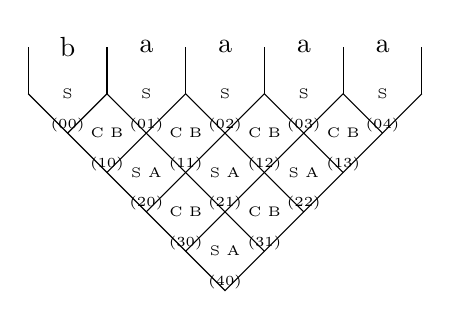
\begin{tikzpicture}[baseline]
				\newcommand{\myfontvars}[1]{
					\fontsize{4.9}{12}\selectfont{#1}
				}\newcommand{\myfontnumbering}[1]{
					\fontsize{2.5}{12}\selectfont{#1}
				}%Outer hull
				%Tip of the pyramid
				\coordinate (tip) at (2.5,-2.5);
				\foreach \i in {0,...,5} {
					\coordinate (\i) at (\i,0);
				}
				%Draw the left and right line of the pyramid pointing downwards
				\draw (0) -- (tip) -- (5);
				%Grid lines direction down-left to top-right
				\coordinate (dl1) at (0.5,-0.5);
				\coordinate (dl2) at (1.0,-1.0);
				\coordinate (dl3) at (1.5,-1.5);
				\coordinate (dl4) at (2.0,-2.0);
				\draw (dl1) -- (1,0);
				\draw (dl2) -- (2,0);
				\draw (dl3) -- (3,0);
				\draw (dl4) -- (4,0);
				%Grid lines direction down-right to top-left
				\coordinate (dr1) at (3.0,-2.0);
				\coordinate (dr2) at (3.5,-1.5);
				\coordinate (dr3) at (4.0,-1.0);
				\coordinate (dr4) at (4.5,-0.5);
				\draw (dr1) -- (1,0);
				\draw (dr2) -- (2,0);
				\draw (dr3) -- (3,0);
				\draw (dr4) -- (4,0);
				%Small lines at the top
				\coordinate (top0) at (0.0,0.0);
				\coordinate (top1) at (1.0,0.0);
				\coordinate (top2) at (2.0,0.0);
				\coordinate (top3) at (3.0,0.0);
				\coordinate (top4) at (4.0,0.0);
				\coordinate (top5) at (5.0,0.0);
				\coordinate (topUpper0) at (0.0,0.6);
				\coordinate (topUpper1) at (1.0,0.6);
				\coordinate (topUpper2) at (2.0,0.6);
				\coordinate (topUpper3) at (3.0,0.6);
				\coordinate (topUpper4) at (4.0,0.6);
				\coordinate (topUpper5) at (5.0,0.6);
				\draw (top0) -- (topUpper0);
				\draw (top1) -- (topUpper1);
				\draw (top2) -- (topUpper2);
				\draw (top3) -- (topUpper3);
				\draw (top4) -- (topUpper4);
				\draw (top5) -- (topUpper5);
				%The string
				\coordinate (w0) at (0.5,0.6);
				\coordinate (w1) at (1.5,0.6);
				\coordinate (w2) at (2.5,0.6);
				\coordinate (w3) at (3.5,0.6);
				\coordinate (w4) at (4.5,0.6);
				\node [] at (w0) {b};
				\node [] at (w1) {a};
				\node [] at (w2) {a};
				\node [] at (w3) {a};
				\node [] at (w4) {a};
				% Variables in the cells
				%cells00
				\coordinate (center00) at (0.5,0.0);
				\node [below=0.18cm] at (center00) {\myfontnumbering{$(00)$}};
				\node [] at (center00) {\myfontvars{S}};
				%cells01
				\coordinate (center01) at (1.5,0.0);
				\node [below=0.18cm] at (center01) {\myfontnumbering{$(01)$}};
				\node [] at (center01) {\myfontvars{S}};
				%cells02
				\coordinate (center02) at (2.5,0.0);
				\node [below=0.18cm] at (center02) {\myfontnumbering{$(02)$}};
				\node [] at (center02) {\myfontvars{S}};
				%cells03
				\coordinate (center03) at (3.5,0.0);
				\node [below=0.18cm] at (center03) {\myfontnumbering{$(03)$}};
				\node [] at (center03) {\myfontvars{S}};
				%cells04
				\coordinate (center04) at (4.5,0.0);
				\node [below=0.18cm] at (center04) {\myfontnumbering{$(04)$}};
				\node [] at (center04) {\myfontvars{S}};
				%cells10
				\coordinate (center10) at (1.0,-0.5);
				\node [below=0.18cm] at (center10) {\myfontnumbering{$(10)$}};
				\node [] at (center10) {\myfontvars{C B}};
				%cells11
				\coordinate (center11) at (2.0,-0.5);
				\node [below=0.18cm] at (center11) {\myfontnumbering{$(11)$}};
				\node [] at (center11) {\myfontvars{C B}};
				%cells12
				\coordinate (center12) at (3.0,-0.5);
				\node [below=0.18cm] at (center12) {\myfontnumbering{$(12)$}};
				\node [] at (center12) {\myfontvars{C B}};
				%cells13
				\coordinate (center13) at (4.0,-0.5);
				\node [below=0.18cm] at (center13) {\myfontnumbering{$(13)$}};
				\node [] at (center13) {\myfontvars{C B}};
				%cells20
				\coordinate (center20) at (1.5,-1.0);
				\node [below=0.18cm] at (center20) {\myfontnumbering{$(20)$}};
				\node [] at (center20) {\myfontvars{S A}};
				%cells21
				\coordinate (center21) at (2.5,-1.0);
				\node [below=0.18cm] at (center21) {\myfontnumbering{$(21)$}};
				\node [] at (center21) {\myfontvars{S A}};
				%cells22
				\coordinate (center22) at (3.5,-1.0);
				\node [below=0.18cm] at (center22) {\myfontnumbering{$(22)$}};
				\node [] at (center22) {\myfontvars{S A}};
				%cells30
				\coordinate (center30) at (2.0,-1.5);
				\node [below=0.18cm] at (center30) {\myfontnumbering{$(30)$}};
				\node [] at (center30) {\myfontvars{C B}};
				%cells31
				\coordinate (center31) at (3.0,-1.5);
				\node [below=0.18cm] at (center31) {\myfontnumbering{$(31)$}};
				\node [] at (center31) {\myfontvars{C B}};
				%cells40
				\coordinate (center40) at (2.5,-2.0);
				\node [below=0.18cm] at (center40) {\myfontnumbering{$(40)$}};
				\node [] at (center40) {\myfontvars{S A}};
				\end{tikzpicture}
			}
		}
	\end{minipage}
	\caption{The simplification of cells in a pyramid.}
	\label{simplificationExample}
\end{figure}

\noindent \textbf{Description of the Algorithm CheckForceCombinationPerCell: }\\
The experience of professor Martens shows that usually most students easily find a pattern of how to fill the first two rows of the $pyramid$ during the execution of the CYK algorithm but do more mistakes starting at row $i\geq2$. Students often don't know exactly what cell combinations need to be considered while filling one specific cell of the pyramid. They simply take only the one top left cell and the one top right cell and try to find rules in the grammar that match the resulting compound variables. The approach of only finding patterns and not thoroughly understanding the algorithm is countered by Algorithm \ref{checkForceCombinationPerCell} CheckForceCombinationPerCell. Here a cell forces if it is possible to see if the student has clearly understood the algorithm and not only take the top left and top right cells.\\

\noindent 
\frame{
	\begin{algorithm}[H] %or another one check
		\caption{CheckForceCombinationPerCell}
		\label{checkForceCombinationPerCell}
		\SetAlgoLined
		\KwIn{$ CellBottom,~CellTopLeft,~CellTopRight \subseteq V,~P \subseteq V \times (V^{2} \cup \Sigma) $ }
		\KwOut{$true \iff |VarsForcing| > 0$}
		$VarsForcing = \emptyset$;~~\tcp{$VarsForcing \subseteq V$} 
		$VarComp = \{xy\ |\ x \in CellTopLeft\ \wedge\ y \in CellTopRight \}$\;
		\ForEach{$v \in CellDown$}{
			$Rhses = \{rhse\ |\ p \in P\ \wedge\ p=(v,rhse)\} $\; \label{rhses}
			\If{$Rhses \nsubseteq VarComp$}{ \label{forces}
				$VarsForcing = VarsForcing \cup v$\;
			}			
		}
		\Return $|VarsForcing| > 0$\;
		\footnotetext{
			Note: $CellBottom=Cell_{i,j}$, $CellUpperLeft=Cell_{i-1,j}$ and  $CellUpperRight=Cell_{i-1,j-1}$\\
			Line \ref{rhses}: Get all rules of $P$ that have $v$ as the $lhse$ and add their $rhse$ to $Rhses$.\\
			Line \ref{forces}: If no $rhse \in Rhse$ can be found in VarComp, then this variables forces, concluding that this cell as a hole forces.
		}
	\end{algorithm}
}

\noindent In the example in Figure \ref{foreCombination}, the variables in $Cell_{2,0}$ and in $Cell_{2,1}$ each force a right cell combination and in both cases $VarComp=\{SS\}$. The variable $v=C$ doesn't have $SS$ as one of its rhses and therefore the variable $C$ forces. $Cell_{3,0}$ does not force because $VarComp=\{CC\}$ and the variable $v=S$ has $CC$ as its rhse. Note again, that cells with index $i\leq1$ can not force at all.
\noindent
\begin{figure} [h]
	\begin{minipage}{6in}
		\centering
		\raisebox{-0.5\height}{
			\begin{tabular}{l}
				$Grammar:$\\
				$C\rightarrow C S~|~a~|~b$\\ 
				$S\rightarrow C C~~$\\ 
			\end{tabular} 
		}
		\hspace*{.2in}
		\raisebox{-0.5\height}{
			\resizebox{0.5\linewidth}{!}{
				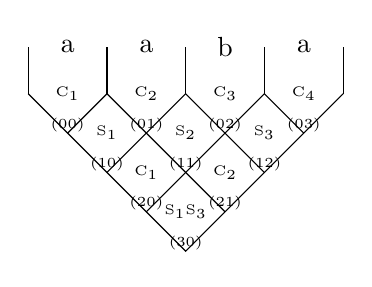
\begin{tikzpicture}[baseline]
				\newcommand{\myfontvars}[1]{
					\fontsize{4.9}{12}\selectfont{#1}
				}\newcommand{\myfontnumbering}[1]{
					\fontsize{2.5}{12}\selectfont{#1}
				}%Outer hull
				%Tip of the pyramid
				\coordinate (tip) at (2.0,-2.0);
				\foreach \i in {0,...,4} {
					\coordinate (\i) at (\i,0);
				}
				%Draw the left and right line of the pyramid pointing downwards
				\draw (0) -- (tip) -- (4);
				%Grid lines direction down-left to top-right
				\coordinate (dl1) at (0.5,-0.5);
				\coordinate (dl2) at (1.0,-1.0);
				\coordinate (dl3) at (1.5,-1.5);
				\draw (dl1) -- (1,0);
				\draw (dl2) -- (2,0);
				\draw (dl3) -- (3,0);
				%Grid lines direction down-right to top-left
				\coordinate (dr1) at (2.5,-1.5);
				\coordinate (dr2) at (3.0,-1.0);
				\coordinate (dr3) at (3.5,-0.5);
				\draw (dr1) -- (1,0);
				\draw (dr2) -- (2,0);
				\draw (dr3) -- (3,0);
				%Small lines at the top
				\coordinate (top0) at (0.0,0.0);
				\coordinate (top1) at (1.0,0.0);
				\coordinate (top2) at (2.0,0.0);
				\coordinate (top3) at (3.0,0.0);
				\coordinate (top4) at (4.0,0.0);
				\coordinate (topUpper0) at (0.0,0.6);
				\coordinate (topUpper1) at (1.0,0.6);
				\coordinate (topUpper2) at (2.0,0.6);
				\coordinate (topUpper3) at (3.0,0.6);
				\coordinate (topUpper4) at (4.0,0.6);
				\draw (top0) -- (topUpper0);
				\draw (top1) -- (topUpper1);
				\draw (top2) -- (topUpper2);
				\draw (top3) -- (topUpper3);
				\draw (top4) -- (topUpper4);
				%The string
				\coordinate (w0) at (0.5,0.6);
				\coordinate (w1) at (1.5,0.6);
				\coordinate (w2) at (2.5,0.6);
				\coordinate (w3) at (3.5,0.6);
				\node [] at (w0) {a};
				\node [] at (w1) {a};
				\node [] at (w2) {b};
				\node [] at (w3) {a};
				% Variables in the cells
				%cells00
				\coordinate (center00) at (0.5,0.0);
				\node [below=0.18cm] at (center00) {\myfontnumbering{$(00)$}};
				\node [] at (center00) {\myfontvars{C$_{1}$}};
				%cells01
				\coordinate (center01) at (1.5,0.0);
				\node [below=0.18cm] at (center01) {\myfontnumbering{$(01)$}};
				\node [] at (center01) {\myfontvars{C$_{2}$}};
				%cells02
				\coordinate (center02) at (2.5,0.0);
				\node [below=0.18cm] at (center02) {\myfontnumbering{$(02)$}};
				\node [] at (center02) {\myfontvars{C$_{3}$}};
				%cells03
				\coordinate (center03) at (3.5,0.0);
				\node [below=0.18cm] at (center03) {\myfontnumbering{$(03)$}};
				\node [] at (center03) {\myfontvars{C$_{4}$}};
				%cells10
				\coordinate (center10) at (1.0,-0.5);
				\node [below=0.18cm] at (center10) {\myfontnumbering{$(10)$}};
				\node [] at (center10) {\myfontvars{S$_{1}$}};
				%cells11
				\coordinate (center11) at (2.0,-0.5);
				\node [below=0.18cm] at (center11) {\myfontnumbering{$(11)$}};
				\node [] at (center11) {\myfontvars{S$_{2}$}};
				%cells12
				\coordinate (center12) at (3.0,-0.5);
				\node [below=0.18cm] at (center12) {\myfontnumbering{$(12)$}};
				\node [] at (center12) {\myfontvars{S$_{3}$}};
				%cells20
				\coordinate (center20) at (1.5,-1.0);
				\node [below=0.18cm] at (center20) {\myfontnumbering{$(20)$}};
				\node [] at (center20) {\myfontvars{C$_{1}$}};
				%cells21
				\coordinate (center21) at (2.5,-1.0);
				\node [below=0.18cm] at (center21) {\myfontnumbering{$(21)$}};
				\node [] at (center21) {\myfontvars{C$_{2}$}};
				%cells30
				\coordinate (center30) at (2.0,-1.5);
				\node [below=0.18cm] at (center30) {\myfontnumbering{$(30)$}};
				\node [] at (center30) {\myfontvars{S$_{1}$S$_{3}$}};
				\end{tikzpicture}
			}
		}
	\end{minipage}
	\caption{Application of Algorithm \ref{checkForceCombinationPerCell} CheckForceCombinationPerCell onto an entire pyramid.}
	\label{foreCombination}
\end{figure}\\

\noindent The three success rates have been explained and finally the overall Success Rate can be specified. \\
\noindent\textbf{Success Rate:}
A generated $exercise$ contributes to the Success Rate (SR) if it contributes to the SR-Producibility, to the SR-Cardinality-Rules and to the SR-Pyramid at the same time.\\
It holds: $SR = n / N$, where $n$ is the count of $exercises$.
\subsubsection{Problem space exploration}
Suitable ranges of parameters, to create exam $exercises$ with, are:
\begin{itemize}[noitemsep,nolistsep]
	\item count of variables = [2;~8]
	\item count of terminals = [2;~8]
	\item size of word = [4;~11]
\end{itemize}
%\vspace{0.6cm}
This input value ranges are used during the further comparison. 
\paragraph{Comparison of the stopping criteria}~\\
As described in Chapter \ref{subModules} Sub Modules, two different stopping criteria \circled{C} are used and it is of interest to know which one helps to generate more suitable exam $exercise$s so that the better one can be used in a real world application. Therefore both variants of the stopping criteria are compared in Table \ref{comparisionMeanValue} and Table \ref{comparisionStoppingCriteria}.

\noindent For every algorithm and for every possible configuration of the input values the SRs are calculated with a batch size N of 1024.

\begin{table}[h]
	\centering
	\begin{tabular}{l|c|c|}
		\cline{2-3}
		& MoreThanHalf & RootNotEmpty \\ \hline
		\multicolumn{1}{|l|}{DiceRollOnly}  & 0.3\%             & \textbf{0.3\%}            \\ \hline
		\multicolumn{1}{|l|}{DiceRollVar1}  & 0.5\%             & \textbf{1.2\%}            \\ \hline
		\multicolumn{1}{|l|}{DiceRollVar2}  & 0.6\%             & \textbf{1.7\%}            \\ \hline
		\multicolumn{1}{|l|}{SplitThenFill} & 1.4\%             & \textbf{1.4\%}            \\ \hline
		\multicolumn{1}{|l|}{SplitAndFill}  & 8.4\%             & \textbf{8.5\%}             \\ \hline
	\end{tabular}
	\caption{Comparison of the mean value of all the configurations of input values for the different algorithms. (N = 1024)}
	\label{comparisionMeanValue}
\end{table}

\noindent Table \ref{comparisionMeanValue} shows the mean value of all the configurations of input values for the different algorithms. In Table \ref{comparisionStoppingCriteria} the best possible SRs of each algorithm are compared.\\



\begin{table}[h]
	\centering
		\begin{tabular}{l|c|c|}
			\cline{2-3}
			& MoreThanHalf & RootNotEmpty \\ \hline
			\multicolumn{1}{|l|}{DiceRollOnly}  & 17\%             & \textbf{17\%}            \\ \hline
			\multicolumn{1}{|l|}{DiceRollVar1}  & 18\%             & \textbf{36\%}            \\ \hline
			\multicolumn{1}{|l|}{DiceRollVar2}  & 20\%             & \textbf{38\%}            \\ \hline
			\multicolumn{1}{|l|}{SplitThenFill} & 36\%             & \textbf{36\%}            \\ \hline
			\multicolumn{1}{|l|}{SplitAndFill}  & 74\%             & \textbf{74\%}             \\ \hline
		\end{tabular}
	\caption{Comparison of the two stopping criteria: Half of the cells in the pyramid are not empty and at least one variable is in the root of the pyramid. (N = 1024)}
	\label{comparisionStoppingCriteria}
\end{table}
\noindent As seen in the two tables above (Table \ref{comparisionMeanValue} and Table \ref{comparisionStoppingCriteria}), the stopping criteria RootNotEmpty performs better or at least equally good in every case. RootNotEmpty wins and all further discussion in the following Chapter \ref{comparisonOfTheAlgorithms} is done with it.
\paragraph{Picking the best algorithm}~\\\label{comparisonOfTheAlgorithms}
\noindent Now that the choice of stopping criteria has been decided in favour of RootNotEmpty, that guarantees the better SRs, it is time to determine the one algorithm that performs the best.\\
As seen in Table \ref{comparisionMeanValue2} the Algorithm \ref{SplitAndFill} SplitAndFill performs the best considering the mean value.

\begin{table}[h]
	\centering
	\begin{tabular}{l|c|}
		\cline{2-2}
														 & RootNotEmpty \\ \hline
		\multicolumn{1}{|l|}{DiceRollOnly}               & \textbf{0.3\%}            \\ \hline
		\multicolumn{1}{|l|}{DiceRollVar1}               & \textbf{1.2\%}            \\ \hline
		\multicolumn{1}{|l|}{DiceRollVar2}               & \textbf{1.7\%}            \\ \hline
		\multicolumn{1}{|l|}{SplitThenFill}              & \textbf{1.4\%}            \\ \hline
		\multicolumn{1}{|l|}{SplitAndFill}               & \textbf{8.5\%}             \\ \hline
	\end{tabular}
	\caption{Comparision of the mean value of all the configurations of input values for the different algorithms with stopping criteria RootNotEmpty. (N = 1024)}
	\label{comparisionMeanValue2}
\end{table}

\noindent The composite success rates of the five algorithms are displayed in more detail in Table \ref{comparisionsAlgorithms}. While looking at the configuration of the algorithms that generate the best SRs, it is seen that the best algorithm for the application to use is Algorithm \ref{SplitAndFill} SplitAndFill, because it has the best SR.

 
\begin{table}[h]
	\centering
	\begin{tabular}{|l|c|c|c|c|c|c|c|}
		\hline
		\multicolumn{1}{|c|}{Algorithm} & SR   & \begin{tabular}[c]{@{}c@{}}Produci-\\ bility\end{tabular} & \begin{tabular}[c]{@{}c@{}}Cardinality-\\ Rules\end{tabular} & \multicolumn{4}{c|}{Pyramid}                                                                                                                                                        \\ \cline{6-8} 
		&      &                                                           &                                                              &      & \begin{tabular}[c]{@{}c@{}}Force-\\ Right\end{tabular} & \begin{tabular}[c]{@{}c@{}}Vars-\\ PerCell\end{tabular} & \begin{tabular}[c]{@{}c@{}}VarsIn-\\ Pyramid\end{tabular} \\ \hline
		DiceRollOnly                    & \textbf{17\%} & 21\%                                                           &98\%                                                              & 47\% &47\%                                                        &100\%                                                         &100\%                                                           \\ \hline
		BottomUpVar1                    &\textbf{36\%}      &60\%                                                           &91\%                                                              &65\%      &69\%                                                        &100\%                                                         &93\%                                                           \\ \hline
		BottomUpVar2                    &\textbf{38\%}      &56\%                                                           &95\%                                                              &69\%      &69\%                                                        &100\%                                                         &100\%                                                           \\ \hline
		SplitThenFill                   &\textbf{36\%}    &51\%                                                           &97\%                                                              &71\%      &71\%                                                        &100\%                                                         &99\%                                                           \\ \hline
		SplitAndFill                    &\textbf{74\%}      &100\%                                                           &100\%                                                              &74\%      &74\%                                                        &100\%                                                         &100\%                                                           \\ \hline
	\end{tabular}
	\caption{More detailed composite $SR$ of the algorithms with their best overall SR. (N = 1024)}
	\label{comparisionsAlgorithms}
\end{table}
\clearpage
\pagebreak